\documentclass[11pt,a4paper,oldfontcommands]{memoir}
\usepackage[utf8]{inputenc}
\usepackage[T1]{fontenc}
\usepackage[nopatch=eqnum]{microtype}
\usepackage{graphicx}
\usepackage{xcolor}
\usepackage{times}
\usepackage{pdfpages}
\usepackage[pdftex]{hyperref}
\usepackage{hypcap}
\usepackage{enumitem}

\usepackage[all,2cell]{xy}
\UseAllTwocells
\usepackage{tikz-cd}

\usepackage[total={210mm,297mm},left=20mm,right=20mm,bindingoffset=10mm,top=25mm,bottom=25mm]{geometry}

%
% Packages e Ambientes
%

\usepackage{amsmath,amssymb,amsthm,mathtools,tensor,bm}
\usepackage{stmaryrd} % para \mapsfrom
\mathtoolsset{showonlyrefs}

\newtheorem{thm}{Theorem}[section]
\newtheorem{prop}[thm]{Proposition}
\newtheorem{coro}[thm]{Corolary}
\newtheorem{lemma}[thm]{Lemma}
\theoremstyle{definition}
\newtheorem{mydef}[thm]{Definition}
\newtheorem{obs}[thm]{Remark}
\newtheorem{example}[thm]{Example}
\newtheorem{examples}[thm]{Examples}
\newtheorem{q}{Question}[section]

\usepackage[english]{babel}

\OnehalfSpacing

%
% Estilos para capítulos e seções
%

\chapterstyle{madsen}
\setsecheadstyle{\Large\bfseries\sffamily\raggedright}
\setsubsecheadstyle{\large\bfseries\sffamily\raggedright}
\setsubsubsecheadstyle{\bfseries\sffamily\raggedright}

%
% Numeração
%

\pagestyle{plain}
\makepagestyle{plain}
\makeevenfoot{plain}{\thepage}{}{}
\makeoddfoot{plain}{}{}{\thepage}
\makeevenhead{plain}{}{}{}
\makeoddhead{plain}{}{}{}

%
% Package para produção do texto em latim para o exemplo do modelo --- pode (talvez deva) ser removido
%

\usepackage{lipsum}
\usepackage{kantlipsum}

%
%  Seus macros
%

\newcommand\NN{\mathbb N}
\newcommand\ZZ{\mathbb Z}
\newcommand\Z{\mathbb Z}
\newcommand\QQ{\mathbb Q}
\newcommand\RR{\mathbb R}
\newcommand\R{\mathbb R}
\newcommand\CC{\mathbb C}
\newcommand\g{\mathfrak g}
\newcommand\U{\mathcal U}
\newcommand\from{\leftarrow}
\newcommand\To{\Rightarrow}
\newcommand\From{\Leftarrow}
\newcommand\xto{\xrightarrow}
\newcommand\xfrom{\xleftarrow}
\newcommand\dashto{\dashrightarrow}
\newcommand\tto{\rightrightarrows}
\newcommand\toto{\rightrightarrows}
\newcommand\acts{\curvearrowright}
\newcommand\res[2]{\left.#1\right|_{#2}}

\DeclareMathOperator{\Ker}{Ker}
\DeclareMathOperator{\coker}{coker}
\DeclareMathOperator{\im}{Im}
\DeclareMathOperator{\id}{id}
\DeclareMathOperator{\Hom}{Hom}
\DeclareMathOperator{\End}{End}
\DeclareMathOperator{\Iso}{Iso}

\DeclareRobustCommand{\2cell}[5]{\xymatrix{#2 \ar@{}[r]|{\Downarrow #5}& #1 \ar@/^.7pc/[l]^{#4} \ar@/_.7pc/[l]_{#3}}}

\newcommand{\red}{\textcolor{red}}
\newcommand{\noi}{\noindent}
\DeclareRobustCommand{\nota}[1]{\marginpar{\flushleft \tiny #1}}
\newcommand{\flechita}{\nota{\red{$\leftarrow$ Acá}}}

\newcommand{\titulo}{TITLE}

% redefinimos \emph para que sea bold
\let\emph\relax
\DeclareTextFontCommand{\emph}{\bfseries}

% line numbers!
\usepackage[pagewise, modulo, mathlines]{lineno}
% \usepackage[pagewise, modulo, displaymath, mathlines]{lineno}
% \usepackage[displaymath, mathlines]{lineno}

\newcommand{\TITULO}{Stacky vector bundles and generalized Grassmannians}
\newcommand{\AUTOR}{Juan Desimoni}
\newcommand{\ORIENTADOR}{Matias L.~del Hoyo}

%%%%%%%%%%%%%%%%%%%%%%%%%%%%%%%%%%%%%%%%%%%%%%%%%%%%%%%%%%%%%%%%%%%%%%%%%%%%%%%%

\begin{document}

%
% Capa
%

\thispagestyle{empty}

{\sffamily\centering\Large


\includegraphics[scale=0.25]{modelo/UFF_brasao.png}

~\vspace{2cm}

Universidade Federal Fluminense

\vspace{\fill}

{\huge\TITULO}

\vspace{3.5cm}

{\LARGE\AUTOR}

\vspace{\fill}


{\large Niterói }


{\large  July 2023}


}

\clearpage

%
% Folha de rosto
%

\thispagestyle{empty}

{\sffamily\centering\Large

~\vspace{\fill}

{\huge\TITULO}

\vspace{3.5cm}

{\LARGE\AUTOR}

\vspace{3.5cm}

{\normalsize\raggedleft
\begin{minipage}{210pt}
Dissertação submetida ao Programa de Pós-Graduação
em Matemática da Universidade Federal Fluminense
como requisito parcial para a obtenção do grau de
Doutor em Matemática.
\end{minipage}
}

\vspace{3.5cm}

Advisor: \ORIENTADOR

\vspace{\fill}

{\large Niterói }


{\large  July 2023}


}

\clearpage

\thispagestyle{empty}

{\centering 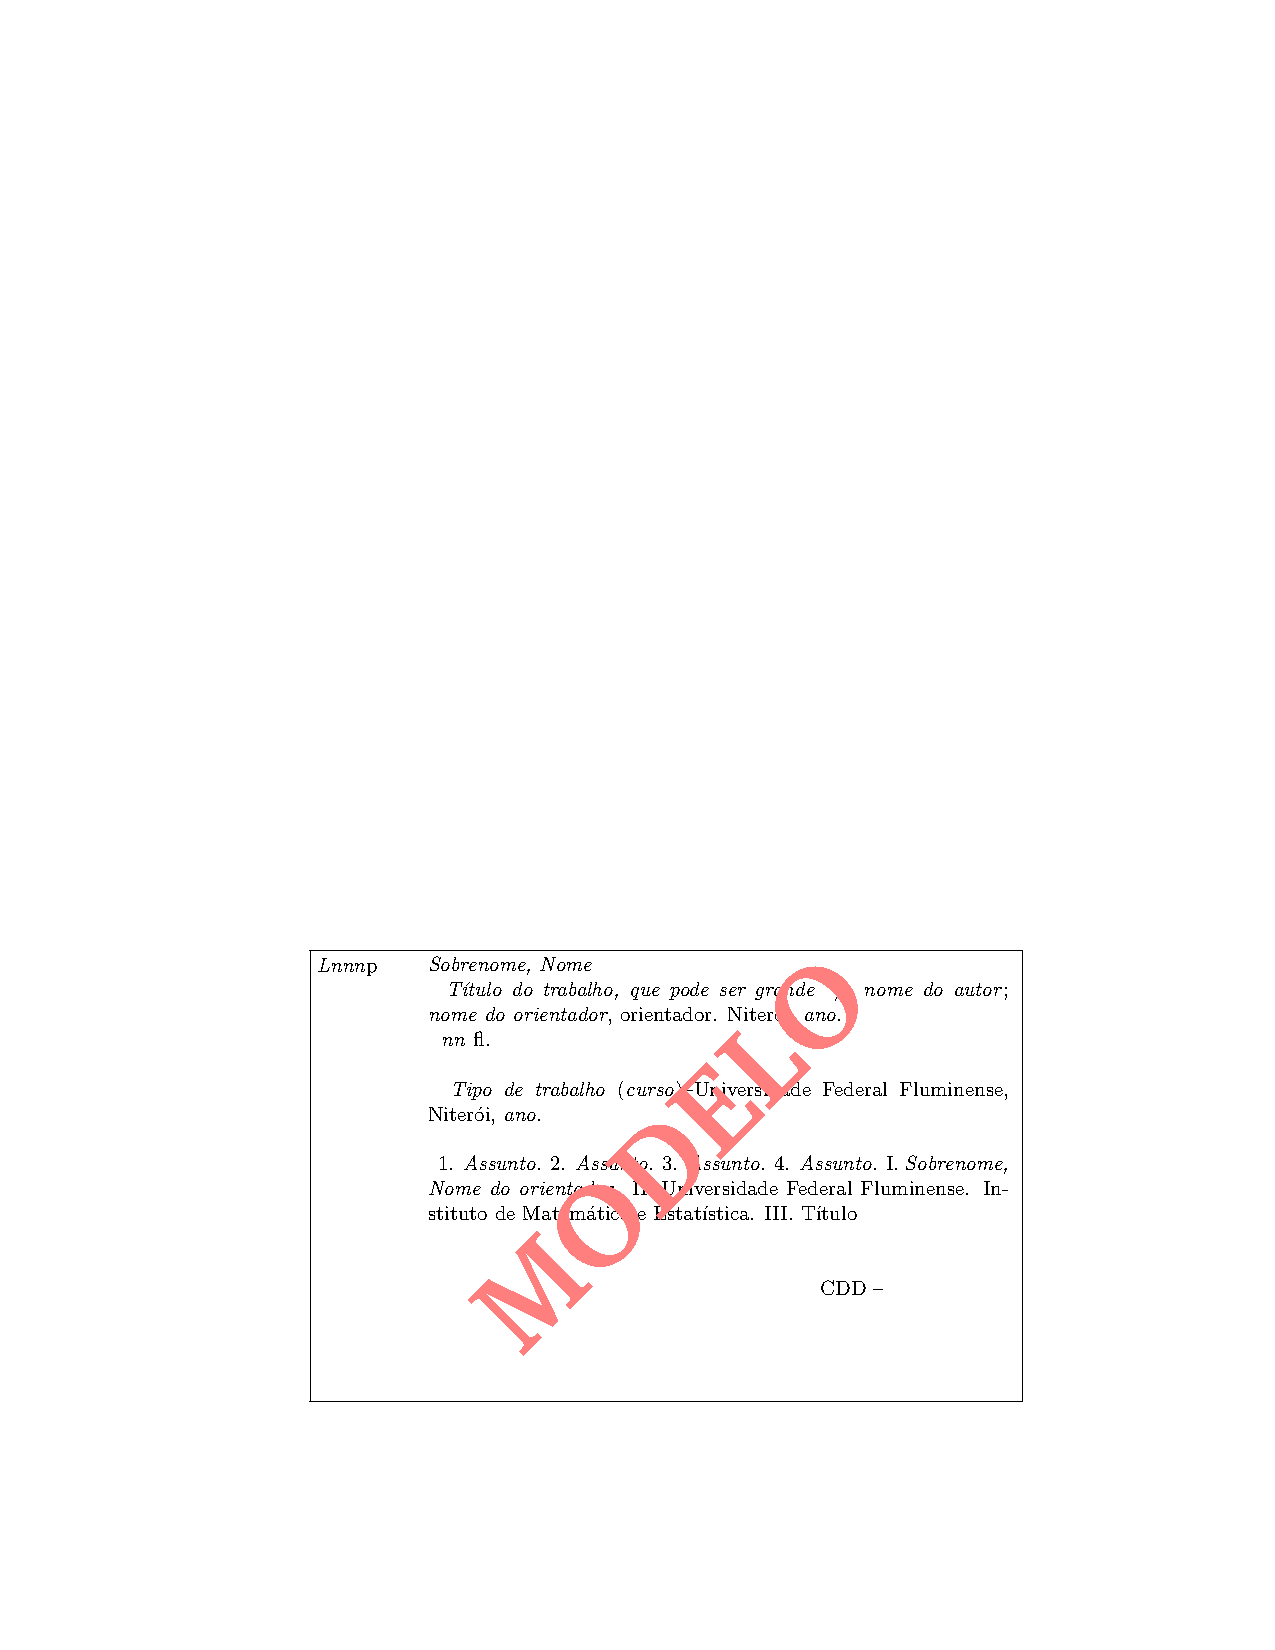
\includepdf{modelo/ficha_catal_modelo}}

\clearpage

\thispagestyle{empty}

{\sffamily\centering

\textbf{Dissertação de Doutorado da Universidade Federal Fluminense}

\vspace{1cm}

 por

\vspace{1cm}

\textbf{\AUTOR}

\vspace{1.5cm}

apresentada ao Programa de Pós-Graduação em Matemática como requesito parcial para a obtenção do grau de

\vspace{1.5cm}

\textbf{Doutor/Mestre em Matemática}

\vspace{1.5cm}

Título da tese:


\hrulefill

\begin{minipage}{0.8\textwidth}
\centering
\textbf{\TITULO}
\end{minipage}
~\vspace{5pt}
\hrule

\vspace{1cm}

\textit{Defendida publicamente em XX julho de 2023.}

\vspace{1cm}

{\raggedright Diante da banca examinadora composta por:}

~\vspace{5pt}

%
% Liste os nomes por ordem alfabética
\begin{tabular}{lll}
  \ORIENTADOR & UFF & Orientador\\
  Simon Chiossi & UFF & Examinador\\
  Thiago Fassarela & UFF & Examinador\\
  Henrique Bursztyn & IMPA & Examinador\\
  Cristián Ortiz & USP & Examinador\\
\end{tabular}

~\vspace{\fill}

}

\clearpage

\thispagestyle{empty}

{
{\centering\textbf{DECLARAÇÃO DE CIÊNCIA E CONCORDÂNCIA DO(A) ORIENTADOR(A)}}

~\vspace{2cm}

Autor(a) da Dissertação: \AUTOR

Data da defesa: XX/07/2023

Orientador(a): \ORIENTADOR

\vspace{2cm}

Para os devidos fins, declaro \textbf{estar ciente} do conteúdo desta \textbf{versão corrigida} elaborada em atenção às sugestões  dos membros da banca examinadora na sessão de defesa do trabalho, manifestando-me \textbf{favoravelmente} ao seu encaminhamento e publicação no \textbf{Repositório Institucional da UFF}.

~\vspace{1cm}

{\raggedright Niterói, XX/03/2023.}

~\vspace{1cm}

\begin{center}
\begin{minipage}{200pt}
\centering
	\hrule

	Nome do orientador(a)
\end{minipage}
\end{center}


}

\clearpage

\thispagestyle{empty}

{

~\vspace{\fill}

\raggedleft
Opcional para esta e aquela pessoa\\
e ainda outra pessoa\\
}

\clearpage

\thispagestyle{empty}

{

\sffamily

{\Large \centering

  AGRADECIMENTOS

}

~\vspace{1cm}

Agradeço a mim mesmo (ou a mais gente). Esta parte é opcional


Agradecimento às agências de fomento --- esta parte \textbf{NÃO É OPCIONAL!}


\textbf{Todas} as teses devem ter o seguinte agradecimento:

\begin{center}
\fbox{
\begin{minipage}{300pt}
O presente trabalho foi realizado com apoio da Coordenação de Aperfeiçoamento de Pessoal de Nível Superior - Brasil (CAPES) - Código de Financiamento 001.
\end{minipage}
}
\end{center}

No caso de bolsa CAPES, sugere-se acrescentar um agradecimento à CAPES pela bolsa. No caso de bolsas de outras agências deve ser verificada quais as regras da agência em particular. Em geral, sugere-se o seguinte: Esse trabalho foi apoiado com uma bolsa de mestrado/doutorado da/do nome da agência, número do processo da bolsa. Outra possibilidade e agradecer a agência em questão a bolsa, mencionando o número do processo ao final.

}

\clearpage

\thispagestyle{empty}

{

	\sffamily

	{\Large	\centering

		RESUMO

	}

~\vspace{1cm}

\lipsum[1-2]

}

\clearpage

\thispagestyle{empty}

{

	\sffamily

	{\Large\centering

		ABSTRACT

	}

~\vspace{1cm}

\kant[1-2]

}


\clearpage
\tableofcontents

% \linenumbers

% \chapter*{Introduction}
% \addcontentsline{toc}{chapter}{Introduction}

\chapter{Lie groupoids}\label{ch:lie-gpds}

\section{First definitions}

%
% SECTION 1 - FIRST DEFINITONS
%

% GROUPOIDS
A \emph{groupoid} $G\tto M$ is a small category in which every arrow is invertible.
It has a set of objects $M=\{x,y,z,\dots\}$ and a set of arrows $G=\{g,h,\dots\}$.
Each arrow $g$ in $G$ has two objects associated to it, the source $s(g)$ and the target $t(g)$.
\[ s,t\colon G\to M  \quad s(y\xfrom{g} x) = x  \quad t(y\xfrom{g} x) = y \]
There is an associative composition law that sends each pair of arrows $g$ and $h$ with $s(h) = t(g)$ to an arrow $hg$ from $s(g)$ to $t(h)$.
Here, by $G\times_M G$ we mean the fiber product between the target and the source maps.
\[ \circ\colon G\times_M G \to G \quad (z\xfrom{h}y, y\xfrom{g}x) \mapsto (z\xfrom{hg}x) \]
For each object $x$ there is a unit arrow \smash{$x\xfrom{u_x} x$}, that satisfies $u_x g = g$ and $h u_x = h$ for every $g$ with $t(g) = x$ and every $h$ with $s(h) = x$.
\[ u\colon M \to G \quad x \mapsto u_x \]
The arrows are required to be invertible, so for each $y\xfrom{g} x$ there is another arrow in the opposite direction $g^{-1}$, satisfying $g^{-1}g = u_x$ and $gg^{-1} = u_y$.
\[ i\colon G \to G \quad g \mapsto g^{-1} \]

% LIE GROUPOIDS
A \emph{Lie groupoid} is a groupoid in which the sets of objects and arrows are manifolds, the structural maps $s$, $t$, $\circ$, $u$ and $i$ are all smooth and the source and target maps are surjective submersions.

As the source and target are left inverses of the unit map, the manifold of objects is an embedded submanifold of the arrows.
With this in mind we will often write $G$ instead of $G\tto M$ to refer to the Lie groupoid in question.
Also note that since the source and target are submersions the domain of the multiplication $G\times_M G$ is a good fiber product (see \cite[\textsection 2.2]{dh13}).

% MORPHISMS OF LIE GPDS
A \emph{morphism} of Lie groupoids $\phi\colon (G\tto M)\to (H\tto N)$ is a smooth functor.
It consists of two smooth maps $M\to N$ and $G\to H$, both denoted again with $\phi$, which commute with the structural maps, that is $s(\phi(g)) = \phi(s(g))$, $t(\phi(g)) = \phi(t(g))$, $\phi(hg) = \phi(h)\phi(g)$, $\phi(u_x) = u_{\phi(x)}$ and $\phi(g^{-1}) = \phi(g)^{-1}$ for every arrow $g\in G$ and every object $x\in M$.
\[
\phi =
\begin{cases}
  G\xto{\phi} H \\
  M\xto{\phi} N
\end{cases}
\]

% EQUIVALENCES
Given two morphisms of Lie groupoids $\phi$ and $\psi$ from $G\tto M$ to $H\tto N$, an \emph{equivalence} $\alpha\colon\phi\Rightarrow\psi$ is a smooth map $\alpha\colon M\to H$ that sends a point $x$ in $M$ to an arrow \smash{$\psi(x)\xfrom{\alpha_x}\phi(x)$}, verifying $\alpha_y \phi(g) = \psi(g) \alpha_x$ for every \smash{$y\xfrom{g} x$} in $G$.
\begin{equation}
\begin{tikzcd}[sep=small]
  \phi(x) \ar{r}{\phi(g)} \ar{d}{\alpha_x} & \phi(y) \ar{d}{\alpha_y} \\
  \psi(x) \ar{r}{\psi(g)} & \psi(y)
\end{tikzcd}
\end{equation}

% ISOTROPY GROUPS
Let us denote by $G(y,x)$ the subset of $G$ consisting of all arrows from $x$ to $y$.
Given an $x\in M$, the \emph{isotropy group} of $G$ at $x$, denoted by $G_x$, is the set $G(x,x)$ of arrows starting and ending at $x$,
%
% ORBITS
and the \emph{orbit} $O_x\subset M$ is the subset of all objects that are connected to $x$ by an arrow.

\medskip\noi \red{DIBUJO. Explicar mejor $\uparrow$.}

% G(y,x)\subset G ARE REGULAR SUBMANIFOLDS
\begin{prop}[\cite{mm03, mack05}]
Given $G\tto M$ and $x,y\in M$, the subset $G(y,x)\subset G$ is an embedded submanifold. In particular $G_x$ is a Lie group. The orbit $O_x\subset M$ is a (maybe not embedded) submanifold in a canonical way. \red{the s-fiber is a principal bundle}
\end{prop}

% ORBIT SPACE M/G
The \emph{orbit space} $M/G$ is set of orbits with the quotient topology
%
% NORMAL SPACES
and the \emph{normal space} $N_xO\subset T_xM$ is the quotient of vector spaces $T_xM/T_xO$.

% ANCHOR
The map $(t,s)\colon G\to M\times M$ is called the \emph{anchor map} of the groupoid.
%
% PROPER AND ÉTALE GPDS
A Lie groupoid with a proper anchor map is a \emph{proper} groupoid.
If the manifolds of objects and arrows $M$ and $G$ have the same dimension, the Lie groupoid $G\tto M$ is said to be \emph{étale}.
%
% TRANSITIVE GPDS
A Lie groupoid is \emph{transitive} if it has a single orbit, or in other words, if for every pair of objects there is an arrow  between them.


\section{Examples of Lie groupoids}

%
% SECTION 2 - EXAMPLES OF LIE GPDS
%

% EX: MANIFOLD
\begin{example}[manifolds]\label{ex:unit}
The \emph{unit groupoid} associated to a manifold $M$ is the Lie groupoid $M\tto M$ whose manifold of arrows has only units and the five structural maps are identities.
Since the morphisms of Lie groupoids should preserve units, a morphism $\phi\colon (M\tto M)\to (N\tto N)$ between pair groupoids is the same as a smooth map $\phi\colon M\to N$.
If $\phi$ and $\psi$ are morphisms between pair groupoids, there is an equivalence $\alpha\colon\phi\Rightarrow\psi$ if and only if they coincide $\phi=\psi$.
For each $x\in M$ the isotropy group at $x$ is $G_x = \{ u_x \}$ and the orbit is $O_x = \{ x \}$.
\end{example}

% EX: OPEN COVER
\begin{example}[open covers]\label{ex:cover}
An open cover $\U=\{U_i\}$ of a manifold $M$ can also be thought of as a Lie groupoid.
The \emph{\v Cech groupoid} \( M_\U = \big( \coprod U_{ji}\tto \coprod U_i \big) \) has the pairs $(x,i)$ with $x\in U_i$ as objects and the triples $(x,j,i)$ with $x\in U_{ji}$ as arrows.
For each $(x,i)$ the isotropy group at $(x,i)$ is $G_{(x,i)}=\{u_{(x,i)}\}$ and the orbit of $(x,i)$ consists of all the $(x,j)$ such that $x$ is in $U_j$.
\end{example}

% EX: PAIR GPD
\begin{example}[pair groupoid]\label{ex:pair}
Let $M$ be a manifold.
A \emph{pair groupoid} $M\times M\tto M$ is a Lie groupoid over $M$ which has one arrow from $x$ to $y$ for every $x,y\in M$.
For each $x\in M$ the isotropy group at $x$ is $G_x = \{(x,x)\}$ and the orbit is $O_x = M$.
Thus, the pair groupoid is transitive.
\end{example}

% EQUIVALENCE RELATION.
\begin{example}[equivalence relations]
Let $R\subset M\times M$ be an \emph{equivalence relation} on a manifold $M$ which is an embedded submanifold and such that the projections onto the first and second factors $\pi_1\colon R\to M$ and $\pi_2\colon R\to M$ are surjective submersions, then $R\tto M$ is a Lie groupoid with trivial isotropy and orbits the equivalence classes.
\end{example}

% EX: LIE GROUPS
\begin{example}[Lie groups]\label{ex:lie-group}
A \emph{Lie group} $G$ is the same as a Lie groupoid over the point $G\tto *$.
The source and target maps are trivial and the multiplication and inversion are given by the Lie group structure.
A morphism of Lie groupoids is the same as a morphisms of Lie groups.
A pair of morphisms of Lie groups from $G$ to $H$ are equivalent if and only if they are related by an inner automorphism.
In other words, there is an equivalence $\alpha\colon\phi\Rightarrow\psi$ if and only if there exists an $h\in H$ such that $\psi=C_h\circ\phi$, where $C_h$ is $C_h(k)=hkh^{-1}$.
We are particularly interested in the General Linear Group $GL_k$, whose manifold of arrows consists of the invertible matrices of rank $k$.
\end{example}

% EX: ACTION GPD
\begin{example}[group actions]\label{ex:action-gpd}
An action of a Lie group $G$ on a manifold $M$ gives rise to an \emph{action groupoid} $G\times M\tto M$ with source $s(g,x) = x$, target $t(g,x) = g\cdot x$ given by the action of $G$, and composition, unit and inverse maps induced by those of $G$.
The orbits and isotropy groups of the action groupoid coincide with the usual notions of orbits and isotropy groups of the action.
\red{Discuss morphisms. In particular it is important that a morphism between the action groupoids need not to come from a morphism between the acting groups, so the functor is not full.}
\end{example}

% EX: VECTOR BUNDLES
\begin{example}[vector bundles]\label{ex:vectorBundle}
A real \emph{vector bundle} of rank $k$ over a manifold $M$ is a locally trivial map $p\colon E\to M$ with fiber $\RR^k$ and structure group $GL_k$.
This means % $p\colon E\to M$ is a surjective submersion where all the fibers are vector bundles of rank $k$, and such
that there are local trivializations $\varphi_i\colon p^{-1}(U_i) \to U_i\times \RR^k$ with $\pi_1\varphi_i=p$, for which the transition maps have the following form \(\varphi_j\varphi_i^{-1}\colon U_{ji}\times\RR^k\to U_{ji}\times\RR^k\), \((x,v)\mapsto (x,\theta_{ji}(x)v)\).
The collection $\{\theta_{ji}\}$ is a \emph{$\bm{GL_k}$-cocycle}, that is, a family of smooth maps $\theta_{ji}\colon U_{ji}\to GL(k,\RR)$ defined over the double intersections such that $\theta_{ii}=1$ and $\theta_{kj}\theta_{ji}=\theta_{ki}$ over the triple intersections.
% Given a cocycle $\theta_{ji}$ defined over an open cover $U_{i}$, it is possible to build a vector bundle \(E=\big( \coprod U_i\times\RR^k \big)/_\sim\), where \((x,i,v)\sim(x,j,\theta_{ji}(x)v)\).
This collection of transition maps $\{\theta_{ji}\}$ constitute a morphism of Lie groupoids from the \v Cech groupoid \( M_\U=\big(\coprod U_{ji}\tto\coprod U_i\big) \) associated to the open cover $\{U_i\}$ of example  \ref{ex:cover} to the General Linear Group $GL_k\tto *$.
% \[ \theta\colon \Big(\coprod U_{ji}\tto \coprod U_i\Big) \to (GL_k\tto *) \qquad  \theta(x,j,i) = \theta_{ji}(x) \]
\end{example}

% EX: G-BUNDLES
\begin{example}[$G$-bundles]
The previous example can be generalized to $G$-bundles.
Let $G$ be a Lie group acting effectively on a manifold $F$, that is, for every pair of distinct $g,h\in G$ there is a $x\in F$ such that $gx\neq hx$.
A \emph{$\bm{G}$-bundle} with fiber type $F$ is a surjective submersion $p\colon E\to M$ together with fiber-preserving diffeomorphisms $\varphi_i\colon p^{-1}(U_i) \to U_i\times F$ defined on an open cover $\{U_i\}$ of $M$, such that the transition functions $\varphi_j\varphi_i^{-1}$ take values in $G$.
The collection of maps \smash{$\res{\varphi_j\varphi_i^{-1}}{\{x\}\times F} = \theta_{ji}\colon U_{ji}\to G$} verify $\theta_{ii}=1$ and $\theta_{kj}\theta_{ji}=\theta_{ki}$, and therefore it is a \emph{$\bm{G}$-cocycle}.
So, by fixing a trivializing open cover $\{U_i\}$, we can think of a $G$-bundle as a morphism of Lie groupoids $\theta\colon\big(\coprod U_{ji}\tto\coprod U_i\big) \to (G\tto *)$, $\theta(x,j,i)=\theta_{ji}(x)$.
\end{example}

% EX: GL(E)
\begin{example}[General Linear Groupoid]\label{ex:gle}
Given\nota{redactar mejor esto} a real vector bundle $E\to M$ of finite rank, there is an associated \emph{General Linear Groupoid}, denoted by $GL(E)\tto M$, which is similar to the General Linear Group associated to a vector space.
Its manifold of objects is $M$ and for any pair of points $x,y\in M$ the arrows between them are the linear isomorphisms between the fibers $\xi\colon E_x\to E_y$.
If\nota{notación? $\varphi_{ji}$} \smash{$\varphi_i\colon \res{E}{U_i} \to \RR^k_{U_i}$} are local trivializations of $E\to M$ defined on open cover $\{U_i\}$ of $M$, then the maps \smash{$\varphi_{ji}\colon GL(E)(U_j)(U_i)\to U_j\times U_i\times\RR^{k^2}$} given by \smash{$\varphi_{ji}(\xi\colon E_x\to E_y)=(y,x,\varphi_j\xi\varphi_i^{-1})$} are charts of $GL(E)$ (see \cite[Example 1.1.12]{mack05}).
\end{example}

% EX: GAUGE GPD
\begin{example}[gauge groupoid]
Let $G$ be a Lie group and $p\colon P\to B$ a principal $G$-bundle, the \emph{gauge groupoid} $P\times^G P\tto B$ is the quotient of the pair groupoid $P\times P\tto P$ by the diagonal diagonal action of $G$.
Gauge groupoids have only one orbit, so, they are transitive.
Conversely, if we start with a transitive groupoid $G\tto M$, we can recover it up to isomorphism as the gauge groupoid associated to the principal $G_x$-bundle $t\colon G(-,x)\to O_x$ for any $x\in M$.
Note that, since a point should be chosen this construction is not functorial.
\end{example}

% EX: SUBMERSION GPD
\begin{example}[submersions]\label{ex:submersion_gpd}
Let $q\colon M\to N$ be a submersion.
The \emph{submersion groupoid} $M\times_N M\tto M$ is the Lie groupoid over $M$ that has an arrow between $x$ and $y$ if and only if they belong to the same fiber of $q$.
The source and target maps are the projections and the composition is $(z,y)\circ(y,x)=(z,x)$.
The orbits of $M\times_N M\tto M$ are the fibers of $q$, the isotropies are trivial and the orbit space identifies with $N$.
Some of the previous examples can also be thought of as submersion groupoids:
the unit groupoid of example \ref{ex:unit} is the submersion groupoid of the identity $\text{id}_M\colon M\to M$,
the pair groupoid, example \ref{ex:pair}, is the submersion groupoid of projection $M\to *$
and the \v Cech groupoid, example \ref{ex:cover}, is the submersion groupoid of the open cover $q\colon\coprod U_i \to M$.
\end{example}


\section{Actions and representations}

%
% SECTION 3 - ACTIONS AND REPRESENTATIONS
%

% ACTIONS
Let $G\tto M$ be a Lie groupoid, $A$ a manifold and $p\colon A\to M$ a map of constant rank.
We denote by $A_x=p^{-1}(x)$ the fiber of $p$ over the point $x$ of $M$.
A (left) \emph{groupoid action} $\theta\colon (G\tto M)\acts (A\to M)$ is a smooth map
\[ \theta\colon G\times_M A\to A \qquad (y\xfrom{g}x, a)\mapsto \theta_g(a) \]
such that $p(\theta_g(a)) = t(g)$, $\theta_{\id}=\id$ and $\theta_{hg}=\theta_h\theta_g$.
Here, by $G\times_M A$ we mean the fiber product between the source map $s\colon G\to M$ and the map $p\colon A\to M$, which is often called the \emph{moment map} of the action.
For each arrow $y\xfrom g x$ there is a diffeomorphism $\theta_g\colon A_x\to A_y$, so, an action is a way of realizing the arrows of the groupoid $G\tto M$ as symmetries of the family of fibers of $p$.

% REPRESENTATIONS
Given a Lie group $G\tto M$ and a vector bundle $E\to M$, a \emph{representation} $\rho\colon (G\tto M)\acts (E\to M)$ is an action in which the maps $\rho_g\colon E_x\to E_y$ are all linear.
% It is given by a smooth map
% $$ \rho\colon G\times_M E\to E \qquad (y\xfrom{g}x, e)\mapsto \rho_g(e) $$
% such that $\pi(\rho_g(e)) = t(g)$, the map $\rho_g\colon E_x\to E_y$ is linear, $\rho_{\id}=\id$ and $\rho_h\rho_g = \rho_{hg}$.
%
% RANK
The \emph{rank} of $\rho$ is defined as the rank of the vector bundle $E\to M$.

%EX: MANIFOLDS
\begin{example}
Let $M$ be a manifold and $E\to M$ a vector bundle.
There is only one representation of the unit groupoid $M\tto M$ on $E\to M$, the trivial one.
So, the representations of a unit groupoid $M\tto M$ are in one-to-one correspondence with the vector bundles over $M$.
\end{example}

%EX: LIE GROUPS
\begin{example}
A vector bundle over the point $V\to *$ is a vector space.
Representations of Lie Groups $(G\tto *)\acts (V\to *)$ are vector spaces equipped with an usual group representation.
\end{example}

%EX: PAIR GPD
\begin{example}
Let $\rho$ be a representation of a pair groupoid $M\times M\tto M$ on a vector bundle $E\to M$.
For any fixed $x_0\in M$ the map $E\to M\times E_{x_0}$, $e\mapsto (x, \rho_{(x_0,x)}(e))$ is a trivialization of $E$.
So, if a vector bundle $E\to M$ admits a representation of the pair groupoid $M\times M\tto M$, then it has to be trivializable.
Conversely, given a global trivialization $\varphi\colon E\to M\times\RR^k$ of $E\to M$, the map $M\times M\times_M E \to E$, $((y,x),x))\mapsto \varphi^{-1}(y,\varphi_2(e))$ is a representation of the pair groupoid $M\times M\tto M$.
\end{example}

Let $\theta\colon (G\tto M)\acts (A\to M)$ be a Lie groupoid action, its \emph{action groupoid} \(G\times_M A\tto A\) is a Lie groupoid over $A$ whose arrows are \smash{$\theta_g(a) \xfrom{(g,a)} a$}.
The source is $s(g,a) = a$, the target $t(g,a) = \theta_g(a)$ is given by the action of $G$, and the composition, unit and inverse maps are induced by those of $G$.
This generalizes example \ref{ex:action-gpd}.
We say that the action $G\acts A$ is \emph{free} if the action groupoid has no isotropy, and that the action is \emph{proper} if the map $G \times_M A \to A\times A$, $(g,a)\mapsto (\theta_g(a),a)$ is so.

% ACTION MAPS
Given an action of Lie groupoids $(G\tto M)\acts (A\to M)$, the moment map $A\to M$ and the projection $G\times_M A\to G$ define a morphisim \((G\times_M A\tto A)\to (G\tto M)\) of particular nature.
Given a constant rank map $p\colon A\to M$, a morphism of Lie groupoids $\phi\colon(H\tto A)\to (G\tto M)$ is an \emph{action map} if it induces a good pullback between the sources.
\begin{equation}
\begin{tikzcd}[sep = small]
  H \ar{r}{s} \ar{d}{\phi} & A \ar{d}{p} \\
  G \ar{r}{s} & M
\end{tikzcd}
\end{equation}

Clearly, the projection \((G\times_M A\tto A)\to (G\tto M)\) associated to an action of Lie groupoids $(G\tto M)\acts (A\to M)$ is an action map.
Conversely, if $(H\tto A)\to (G\tto M)$ is an action map, then $H$ is diffeomorphic to $G\times_M A$ and the composition \smash{$G\times_M A\to H\xto t A$} is an action, it is called the \emph{underlying action}.
It is straightforward to check that these constructions are mutually inverse.

\begin{prop}[\cite{mack05}]
There is a one-to-one correspondence between left actions and action maps.
\end{prop}

% AS A MAP FROM G TO GL(E)
If $\rho\colon G\times_ME\to E$ is a representation, for each arrow $y\xfrom g x$ there is an isomorprism of vector bundles $\rho_g\colon E_x\to E_y$, which is an element of the General Linear Groupoid described in example \ref{ex:gle}.
So, one could alternatively define a representation as a morphism of Lie groupoids $(G\tto M)\to (GL(E)\tto M)$ that is the identity over $M$.
In fact, both definitions are equivalent.

\begin{prop}\label{repr}
There is a one-to-one correspondence between representations of $G\tto M$ over $E\to M$ and Lie groupoid maps from $G\tto M$ to the General Linear Groupoid $GL(E)$
% \[ rho\colon (G\tto M)\to (GL(E)\tto M) \qquad g \mapsto \rho_g \]
that are the identity over $M$.
\end{prop}

\begin{proof}
Given a representation $\rho\colon G\times_ME\to E$, let us consider the morphism of groupoids $\psi\colon(G\tto M)\to(GL(E)\tto M)$ that is the identity over $M$ and sends an arrow \smash{$y\xfrom{g} x$} to the linear isomorphism \smash{$\rho_g\colon E_x\to E_y$}.
To see that the morphism $\psi$ is smooth, let us pick a chart \smash{$\varphi_{ji}\colon GL(E)(U_j)(U_i)\to U_j\times U_i\times\RR^{k^2}$} of $GL(E)$ (see example \ref{ex:gle}) and consider the composition \smash{$\varphi_{ji}\res{\psi}{G(U_j,U_i)}\colon G(U_j,U_i)\to U_j\times U_i\times\RR^{k^2}$}.
By looking at the last factor we have a map \smash{$A\colon G(U_j,U_i)\to \RR^{k^2}$} that assigns the matrix \smash{$A(g)=\varphi_j\rho_g\varphi_i^{-1}\in\RR^{k^2}$} to each arrow $g\in G(U_j,U_i)$.
Let $\{e_1,\dots,e_k\}$ be the canonical basis of $\RR^k$ and $\{e^1,\dots,e^k\}$ its dual basis.
For each $1\leq r,s\leq k$ the entry $rs$ of $A$ is $A{rs}=e^s\circ\varphi_j\circ\rho\circ\varphi_i^{-1}\circ i_{e_r}$,
which is a smooth function of $g$.
Here, $i_{e_r}\colon G\to G\times\RR^k$ is $g\mapsto(g,e_r)$,
Therefore, \smash{$A\colon G(U_j,U_i)\to \RR^{k^2}$} is smooth and so is $\psi\colon G\to GL(E)$.
This shows that we have a well defined morphism of Lie groupoids $\psi\colon(G\tto M)\to(GL(E)\tto M)$.

Conversely, if we have a morphism of Lie groupoids $\psi\colon(G\tto M)\to(GL(E)\tto M)$, let $\rho\colon G\times_ME\to E$ be the map given by $\rho(g,e)=\psi_g(e)$.
As $\psi$ is a morphism of groupoids, $\rho$ is an action.
To see that it is smooth, note that $\rho=\text{ev}\circ(\psi\times \text{id}_E)$, where $\text{ev}\colon GL(E)\times_M E\to E$ is the evaluation $\text{ev}(\xi,e)=\xi(e)$.
\end{proof}

If one tries to carry on the characterization of Proposition \ref{repr}, but for actions in general instad of representations, the resulting space is infinite dimensional.
\red{Should be developed. Explain the set-theoretic situation and the smooth aspects.}

% MORPHISMS OF REPRESENTATIONS
If\nota{subir esto?} $\rho_1\colon (G\tto M)\acts (E_1\to M)$ and $\rho_2\colon (G\tto M)\acts (E_2\to M)$ are representations of the same groupoid $G\tto M$, a \emph{morphism} $\eta\colon \rho_1 \Rightarrow \rho_2$ between them is a morphism of vector bundles $\eta\colon E_1 \to E_2$ such that $\eta_y\rho_1(g) = \rho_2(g)\eta_x$ for every arrow $y\xfrom{g}x$ of $G$.

% PULLBACK OF REPRESENTATIONS
Let $\rho\colon (G\tto M)\acts (E\to M)$ be a representation.
Given another Lie groupoid $H\tto N$ and morphism $\phi\colon (H\tto N) \to (G\tto M)$, we can consider the \emph{pull-back} of $\rho$ via $\phi$, denoted by \(\phi^*(\rho)\colon (H\tto N)\acts (\phi^*E\to N)\).
This is a representation of $H\tto N$ on the pull-back vector bundle $\phi^*E\to N$ that sends an arrow \smash{$w\xfrom h z$} to the linear isomorphism $\rho(\phi(h))\colon E_{\phi(w)}\to E_{\phi(z)}$.

% EX: VECTOR BUNDLES AS REPRESENTATIONS
\begin{example}
In example \ref{ex:vectorBundle} we observed that, by picking a trivializing open cover $\U=\{U_i\}$ of the base, a vector bundle of rank $k$ over $M$ can be seen a morphism of Lie groupoids $\theta\colon M_\U \to GL_k$.
Considering the pull-back of the identity representation of $GL_k$ on $\RR^k$ via the morphism $\theta$, we can also think of a vector bundle, or a $GL_k$-cocycle, as a representation of the \v Cech groupoid $M_\U$ on the pull-back vector bundle $\theta^*(\RR^k) = \big( \coprod U_i\times \RR^k \to \coprod U_i \big)$.
\end{example}

\red{Write example on submersion groupoids, it works exactly as the open cover case, it is called ``descent theory'', read wikipedia article about it.}

% % En realidad esta proposición son dos:
% % 1) El pull-back de representaciones es funtorial
% % 2) Si $\phi_1$ y $\phi_2$ son morfismos de fibrados naturalmente equivalentes, entonces $\phi_1^* = \phi_2^*$.
% \begin{prop}\label{iso}
% Let $\phi_1$ and $\phi_2$ be morphisms of Lie groupoids from $G'\tto M'$ to $G\tto M$ and $\rho_1\colon (G\tto M)\to (GL(E_1)\tto M)$ and $\rho_2\colon (G\tto M)\to (GL(E_2)\tto M)$ two representations of $G\tto M$.
% % If $\phi_1\simeq\phi_2$ and $\rho_1\simeq\rho_2$, then $\phi_1^*\rho_1 \simeq \phi_2^*\rho_2$.
% If the morphisms $\phi_1$ and $\phi_2$ are naturally equivalent and the representations $\rho_1$ and $\rho_2$ are isomorphic, then so are $\phi_1^*\rho_1$ and $\phi_2^*\rho_2$.
% \end{prop}

% \begin{proof}
% Let $\eta\colon E_1\to E_2$ be an isomorphism of vector bundles providing the isomorphism $\rho_1\simeq\rho_2$ and let $\alpha$ be a natural equivalence $\phi_1\simeq\phi_2$.
% Given an $x'\in M'$, let $\mu_{x'}\colon \left(\phi_1^*E_1\right)_{x'} \to \left(\phi_2^*E_2\right)_{x'}$ be the isomorphism of vector spaces defined by $\mu_{x'} = \eta_{\phi_2(x')}\rho_1(\alpha_{x'})$.
% This gives us a section of the fiber bundle $\Iso\left(\rho_1^*E_1,\rho_2^*E_2\right)$ such that $\mu_{y'}\rho_1(\phi_1(g')) = \rho_2(\phi_2(g'))\mu_{x'}$ for every arrow $g'\colon x'\to y'$ of $G'$.
% \end{proof}

% \begin{prop}\label{morita}
% If $\phi\colon (G\tto M) \to (G'\tto M')$ is a Morita morphism such that the map on the objects $\phi\colon M\to M'$ is a surjective submersion, then the pull-back induces a bijection between the sets of isomorphism classes of representations of $G\tto M$ and of $G'\tto M'$.
% \end{prop}

% \begin{proof}
% As the morphism $\phi$ is a surjective submersion on the objects, choosing local sections we can obtain an open cover $\U'$ and a morphism $\sigma\colon G'_{\U'} \to G$ such that $\pi'_{\U'} = \phi\sigma$.
% Consider the cover $\U$ of $M$ that has all the preimages via $\phi$ of all the open sets $U'$ in $\U'$.
% We have the following commutative diagram.
% \begin{equation*}
% \begin{tikzcd}
%  G_\U \ar{r}{\pi_\U} \ar{d}[swap]{\phi_\U} & G \ar{d}{\phi} \\
%  G'_{\U'} \ar{r}[swap]{\pi'_{\U'}} \ar{ur}{\sigma} & G'
% \end{tikzcd}
% \end{equation*}
% Observing that $\sigma^*\phi^* = \pi'^*_{\U'}$ and $\phi_\U^*\sigma^* = \pi_\U^*$ we get that if $\pi'^*_{\U'}$ and $\pi^*_\U$ induce bijections between the respective sets of representations, then so does $\phi^*$.
% Hence, it is enough to prove that the result holds for a morphism of Lie groupoids of the form $\pi_\U\colon G_\U \to G$.

% If $\rho_1\colon (G\tto M) \to (GL(E_1)\tto M)$ and $\rho_2\colon (G\tto M) \to (GL(E_2)\tto M)$ are two representations of $G\tto M$ such that the pull-backs $\pi_\U^*(\rho_1)$ and $\pi_\U^*(\rho_2)$ are isomorphic, let us say, via an isomorphism of vector bundles $\mu\colon\pi_\U^*(E_1) \to \pi_\U^*(E_2)$.
% Putting $\eta_i(x) = \mu_{(x,i)}$ we have a family of isomorphisms of vector bundles $\eta_i\colon \res{E_1}{U_i} \to \res{E_2}{U_i}$.
% Note that $\eta_i(x) = \pi_\U^*\rho_2(u_x,i,j) \, \mu_{(x,i)} = \mu_{(x,j)} \, \pi_\U^*\rho_1(u_x,i,j) = \eta_j(x)$ for every $x \in U_{ij}$.
% This allows us to glue the $\eta_i$ all together to get a morphism of vector bundles $\eta\colon E_1 \to E_2$ that gives us the desired isomorphism of representations between $\rho_1$ and $\rho_2$.
% This proves the injectivity of $\pi_\U^*$.

% For the surjectivity, given a representation $\tau\colon (\coprod_{i,j} G(U_i,U_j) \tto \coprod_i U_i) \to (GL(F)\tto \coprod_i U_i)$ of $G_\U$, let us consider the vector bundle $E = ( \coprod_i F_{(x,i)} ) / _\sim$, where we are identifying a $v$ in the fiber $F_{(x,i)}$ with $\tau(u_x,i,j) \, v$ in $F_{(x,j)}$ for every $j$ such that $x$ also belongs to $U_j$.
% The representation $\rho\colon (G\tto M) \to (GL(E)\tto M)$ of $G$ that sends an arrow $g\colon x\to y$ to the isomorphism $\rho\colon E_x \to E_y$ induced by $\tau(g,i,j)\colon F_{(x,i)} \to F_{(x,j)}$ where $i$ and $j$ are any such that $x$ is in $U_i$ and $y$ is in $U_j$, satisfies that $\pi_\U^*(\rho) = \tau$.
% \end{proof}

% \begin{thm}
% The pull-back of representations induces a natural bijection between the set of maps of stacks from a manifold $M$ to the classifying stack of the general linear groupoid $BGL(k,\CC)$ and the set of isomorphism classes o rank $k$ vector bundles over $M$.
% \end{thm}

% \begin{proof}
% Let us use $G\tto *$ as an abbreviation for the general linear group $GL(k,\CC)$.
% If we are given a map of stacks from $M$ to $BG$, let us say represented by a fraction
% \begin{equation*}
% \begin{tikzcd}
%  (M\tto M) & (H\tto N) \ar{l}[sloped, below]{\sim}[sloped, above]{\phi} \ar{r}{\psi} & (G\tto *) ,
% \end{tikzcd}
% \end{equation*}
% we can pull-back the identity representation of $G\tto *$ to obtain a representation of $H\tto N$, let us call it $\tau$.
% As the map $\phi$ is Morita and a surjective submersion on the objects, by proposition \ref{morita} we know that there exists a unique (modulo isomorphism) representation $\rho\colon (M\tto M) \to (GL(E)\tto M)$ such that that $\phi^*\rho$ and $\tau$ are isomorphic.
% Propositions \ref{iso} and \ref{morita} together with the observations made in example \ref{rep-unit} assure us that we have a well defined mapping $\psi/\phi \mapsto [E\to M]$, that does not depend on the choice of the representative $(\psi,\phi)$.
% Let us denote this mapping with $\psi/\phi \mapsto (\psi/\phi)^*(1) = [E\to M]$.

% By lemma \ref{representative}, we can choose a representative of the form of the form $\theta/\pi_\U$ for some open cover $\U$ of $M$.
% To have an isomorphims class of vector bundles $[E\to M]$ is the same as an equivalence class of cocycles $[(\U,\{\theta_{ij}\})]$, and this is the same as a map of stacks $\theta/\pi_\U$.

% \noi FALTA TERMINAR.
% \end{proof}


\section{Nerve and cohomology}

%
% SECTION 4 - NERVE AND COHOMOLOGY
%

% NERVE
The \emph{nerve} of a Lie groupoid $G\tto M$, denoted $NG$, is the simplicial manifold whose $k$-simplices $N_kG$ are the strings of composable arrows $(g_k,\dots,g_1)$ such that $s(g_{i+1}) = t(g_i)$ for all $1\leq i\leq k-1$.
So, $N_0G = M$, $N_1G = G$, $N_2G = G\times_M G$ and so on.
\[ (g_k,\dots,g_1) \colon x_k \leftarrow \dots \leftarrow x_i \xfrom{g_i} x_{i-1} \leftarrow \dots \leftarrow x_0 \]
The \emph{face maps} $d_i\colon N_kG \to N_{k-1}G$ are $d_1=s$ and $d_0=t$ for $k=1$, and
\begin{equation}
d_i(g_k,\dots,g_1) =
\begin{cases}
  (g_k,\dots,g_2) & i = 0 \\
  (g_k,\dots,g_{i+1}g_i,\dots,g_1) & 1 \leq i \leq k-1 \\
  (g_{k-1},\dots,g_1) & i = k
\end{cases}
\end{equation}
for $k>1$.
The \emph{degeneracies} $s_j\colon N_kG \to N_{k+1}G$ are
\begin{equation}
s_j(g_k,\dots,g_1) =
\begin{cases}
  (g_k,\dots,g_1,u_{s(g_1)}) & j = 0 \\
  (g_k,\dots,g_{j+1},u_{t(g_j)},g_j,\dots,g_1) & 1 \leq j \leq k . \\
\end{cases}
\end{equation}
% A $k$-simplex is \emph{degenerated} if it is in the image of one of the degeneracies.

% DIFFERENTIABLE COHOMOLOGY
Considering the functions on the manifolds of $k$-simplices and the differentials
\[ \delta\colon C^\infty(N_kG)\to C^\infty(N_{k+1}G) \qquad \delta = \sum_{i=0}^{k+1} (-1)^{k+1-i} \, d_i^* \]
we get the \emph{differentiable complex} $(C^\infty(NG), \delta)$.
\[ C^\infty(NG)\colon \quad C^\infty(M) \xto{\delta} C^\infty(G) \xto{\delta} C^\infty(G\times_M G) \xto{\delta} \cdots \]
Its cohomology $H_\text{diff}^*(G)$  is the \emph{differentiable cohomology} of the Lie groupoid $G\tto M$.

% NON-REDUCED BOTT-SHULMAN COMPLEX
For each $k$, we can also consider the $l$-forms on the manifolds of $k$-simplices together with the maps
\[ \delta\colon \Omega^l(N_kG)\to \Omega^l(N_{k+1}G) \qquad \delta = \sum_{i=0}^{k+1} (-1)^{i+l} \, d_i^* \]
to get the chain complexes $(\Omega^l(NG), \delta)$.
\[ \Omega^l(NG)\colon \quad \Omega^l(M) \xto{\delta} \Omega^l(G) \xto{\delta} \Omega^l(G\times_M G) \xto{\delta} \cdots \]
If we also take the De Rham cohomology into acount we get a double complex, the (non-reduced) \emph{Bott-Shulman complex}:
\begin{equation}
\begin{tikzcd}[sep = small]
  \vdots & \vdots & \vdots \\
  \Omega^2(M) \ar{u} \ar{r}{\delta} & \Omega^2(G) \ar{u} \ar{r}{\delta} & \Omega^2(N_2G) \ar{u} \ar{r} & \cdots \\
  \Omega^1(M) \ar{u}{d} \ar{r}{\delta} & \Omega^1(G) \ar{u}{d} \ar{r}{\delta} & \Omega^1(N_2G) \ar{u}{d} \ar{r} & \cdots \\
  C^\infty(M) \ar{u}{d} \ar{r}{\delta} & C^\infty(G) \ar{u}{d} \ar{r}{\delta} & C^\infty(N_2G) \ar{u}{d} \ar{r} & \cdots
\end{tikzcd}
\end{equation}
%
% REDUCED BOTT-SHULMAN COMPLEX
The degenerated simplices, that is, the ones that are in the image of the degeneracies, will not be of interest for us.
So, we will replace the spaces of $l$-forms $\Omega^l(N_kG)$ with the ones that are zero on the degenerated simplices.
\begin{equation}
K^{k,l}(G\tto M) =
\begin{cases}
    \Omega^l(M) & k = 0 \\
    \bigcap_{i=0}^{k-1} \Ker\left( s_i^*\colon \Omega^l(N_kG) \to \Omega^l(N_{k-1}G) \right) & k > 0
\end{cases}
\end{equation}
The resulting complex $(K^{*,*}(G),\delta,d)$ is knwown as the \emph{reduced Bott-Shulman complex} of the Lie groupoid $G$.
%
% COHOMOLOGY OF LIE GROUPOIDS
The cohomology of $G\tto M$ is defined as the cohomology of the total complex of $(K^{*,*}(G), d, \delta)$.
\[ H^*(G) = H^*(\text{Tot}(K^{*,*}(G))) \]

It is worth noting that both constructions, the reduced and the non-reduced version of the Bott-Shulman, yield equivalent complexes.
Since it is more convenient to cross out the degenerated simplices, we will prefer the reduced version over the non-reduced one.

\begin{example}
Let $M\tto M$ be a unit groupoid, its the Bott-Shulman complex has zeros everywhere except for the first column.
So, the Bott-Shulman complex of a manifold is the De Rham complex.
\end{example}

\begin{example}
Let $M_\U$ be the \v{C}ech grupoid of a manifold $M$ with an open cover $\U$ that we presented in example \ref{ex:cover}.
The (reduced) Bott-Shulman complex of $M_\U$ is the \v{C}ech-de Rham complex (see \cite[chapter 2]{bott-tu}).
\end{example}

\begin{example}
Let $G\tto *$ be a Lie group, then $N_0G=*$, $N_1G=G$, $N_2G=G\times G$ and so on.
In this case the differentiable cohomology is the group cohomology of $G$, and the Bott-Shulman complex ???
\end{example}

\begin{example}
Let $(G\tto M)\acts(A\to M)$ be an action of Lie groupoids and let $G\times_M A\tto A$ be the corresponding action groupoid. ???
\end{example}

% ME GUSTARIA ENCONTRAR LA FORMA DE PONER ESTO
% \begin{prop}[Grothendieck]
% A\nota{acá hay que\\ definir un montón\\ de cosas antes} simplicial object $X_\bullet \in sC$ is isomorphic to the nerve of a Lie groupoid if and only if the maps
% $$ \lambda_i^k\colon X_k\to \Lambda_i^k $$
%   are covers for $k=1$ and isomorphisms for $k>1$.
% \end{prop}




% % DIFFERENTIAL COHOMOLOGY WITH COEFFICIENTS IN A REPRESENTATION
% Let us consider the maps
% \begin{align*}
% G_k &\xto{s} M \\
% (g_1,\dots,g_k) &\mapsto x_0 = s(g_1) \text{.}
% \end{align*}
% Given a vector bundle $E$ over $M$, let $C(G_k,E)$ be the vector space of sections of the pull-back $s^*E$.
% An element of $C(G_k,E)$ is a smooth map $\sigma\colon G_k\to E$ such that $\sigma(g_1,\dots,g_k)$ belongs to the fiber $E_{x_0}$.
% Let $C(G,E)$ be the direct sum $\bigoplus_{k\geq 0} C(G_k,E)$.
% If $\rho\colon G\to GL(E)$ is a representation of $G\tto M$ we can consider the maps
% $\delta_\rho\colon C(G_k,E)\to C(G_{k+1},E)$
% given by
% \begin{equation*}
% \delta_\rho(\sigma)(g_1,\dots,g_{k+1}) = \rho_{g_1}^{-1} d_0^*(\sigma)(g_1,\dots,g_{k+1}) + \sum_{i=1}^{k+1} (-1)^i \, d_i^*(\sigma)(g_1,\dots,g_{k+1}) \text{.}
% \end{equation*}
% \begin{lemma}
% The mapping $\rho \mapsto \delta_\rho$ induces a bijection between the representations $\rho\colon G\to GL(E)$ and the degree $1$ differential operators $\delta_\rho\colon C(G,E)\to C(G,E)$ with square zero.
% \end{lemma}

% Observe that when $E$ is the trivial line bundle $M\times\CC$ and $\rho$ is the trivial representation, we have that $(C(G,E),\delta_\rho)$ is the complex $(C^\infty(G_*),\delta)$ defined above.

% Given a vector bundle $E\to M$ and a representation $\rho\colon G\to GL(E)$, we define the \emph{differential cohomology with coefficients} in the representation $\rho$, denoted $H^*(G,E)$, to be the cohomology of the complex $(C(G,E),\delta_\rho)$.\\

% % COADJOINT REPRESENTATION OF A LIE GROUP
% Let us breafly recall the coadjoint representation of a Lie group $G\tto *$, it is given by the map
% \begin{align*}
% G &\to GL(\g^*) \\
% g &\mapsto \text{ad}_g
% \end{align*}
% where $\text{ad}_g(\xi)(X_e) = \xi(d_e\rho_{g^{-1}}(X_e))$ for every $\xi\in \g^*$ and $X_e\in \g$, and $\rho_g$ is the conjugation by the element $g$ of $G$.

% BOTT MANAGED TO COMPUTE THE HORIZONTAL COHOMOLOGIES OF THE BOTT-SHULMAN COMPLEX
%   $H_\delta ^p(\Omega^q(G_*) \simeq H_\text{diff}^{p-q}(G, S^q(\mathfrak{g}^*))$

% BOTT'S SPECTRAL SEQUENCE: E_{pq}^1 => H^{p+q}(BG)

% IF G IS A COMPACT LIE GROUP, THEN H^{p+q}(BG) = 0 if p \neq q
%   AND H^{2p}(BG) = S^q(\mathfrak{g}^*)^G










%%%%%%%%%%
%%%%%%%%%%

\chapter{VB-groupoids}\label{ch:vb-gpds}

\section{Definitions and basic facts}\label{sec:VBgpds}

%
% SECTION 1 - DEFINITIONS AND BASIC FACTS
%

% VB-GPDS
A \emph{VB-groupoid} $\Gamma\tto E$ over a Lie groupoid $G\tto M$, sometimes denoted simply by $\Gamma$, consists of Lie groupoids $\Gamma\tto E$, $G\tto M$ and a morphism $(\Gamma\tto E)\to (G\tto M)$ such that the maps on the arrows $\Gamma\to G$ and on the objects $E\to M$ are vector bundle projections for which the structure maps of $\Gamma\tto E$ are linear \cite{mack05}.
\begin{equation}
\begin{tikzcd}[sep=small, cells={text width={width("$M$")}}, align=center]
  \Gamma \ar[yshift=3pt]{r} \ar[yshift=-2.3pt]{r} \ar{d} & E \ar{d} \\
  G \ar[yshift=3pt]{r} \ar[yshift=-2.3pt]{r} & M
\end{tikzcd}
\end{equation}

% CORE, SIDE AND ANCHOR MAP
Given a VB-groupoid $(\Gamma\tto E)\to (G\tto M)$, its \emph{core bundle} is $C=\ker(s\colon\res{\Gamma}{M}\to E)$, the \emph{anchor map} is $\partial=\res{t}{C}\colon C\to E$ and the vector bundle $E\to M$ is called the \emph{unit bundle}.

% MORPHISMS
A \emph{morphism} of VB-groupoids $\Phi\colon\Gamma\to\Gamma'$ is a Lie groupoid morphism $\Phi\colon(\Gamma\tto E)\to(\Gamma'\tto E')$ covering another $\phi\colon(G\tto M)\to (G'\tto M')$ such that $\phi$ is fiberwise linar.
When $G'=G$ and $\varphi$ is the identity we say that $\phi$ is a morphism over $G$.

% LINEAR EQUIVALENCE
Given \nota{revisar esto. relacionar con equivalencias de mapas de Lie gdps.} two morphisms of VB-groupoids $\Phi,\Psi\colon\Gamma\to \Gamma'$ over $G$, a \emph{linear equivalence}
$\alpha\colon\Phi\Rightarrow\Psi$ is a vector bundle map \smash{$\alpha\colon E\to\res{\Gamma'}{M}$} covering the identity of $M$
that sends an $e\in E$ to an arrow \smash{$\psi(e)\xfrom{\alpha_e}\phi(e)\in\res{\Gamma'}{M}$} such that $\alpha_{\tilde e} \Phi(\gamma) = \Psi(\gamma) \alpha_e$ for every \smash{$\tilde e\xfrom{\gamma} e\in \Gamma$}.

% VB-GPD DERIVED CATEGORY
We denote by $\mathrm{VB}(G\tto M)$ the category of VB-groupoids over $G\tto M$ with the morphisms covering the identity, and with $\mathrm{VB}[G\tto M]$ the \emph{derived category} of VB-groupoids over $G\tto M$, that is obtained from $\mathrm{VB}(G\tto M)$ by identifying equivalent morphisms.
The objects of $\mathrm{VB}[G\tto M]$ are the VB-groupoids over $G\tto M$ and the arrows are the equivalence classes of morphisms over $G\tto M$.
Note that an isomorphism in the derived category $\mathrm{VB}[G\tto M]$ is given by a morphism $\phi$ that admits an inverse up to linear equivalence.

% EX: 2-VECT
\begin{example}\label{ex:2vect}
A VB-groupoid over the point $*\tto *$ is a \emph{2-vect} in the sense of \cite{bc04}.
\begin{equation}
  \begin{tikzcd}[sep=small, cells={text width={width("$M$")}}, align=center]
    V_1 \ar[yshift=3pt]{r} \ar[yshift=-2.3pt]{r} \ar{d} & V_0 \ar{d} \\
    * \ar[yshift=3pt]{r} \ar[yshift=-2.3pt]{r} & *
  \end{tikzcd}
\end{equation}
Equivalently, a 2-vect is a category object in the category of vector spaces.
It consists of a vector space of objects $V_0$ and a vector space of morphisms $V_1$, such that the source and target maps $s, t\colon V_1\to V_0$, the identity $i\colon V_0\to V_1$ and the composition $\circ\colon V_1\times_{V_0}V_1\to V_1$ are all linear.
By Dold-Kan correspondence, a 2-vect is completely encoded in its anchor map $\partial\colon V_1\to V_0$.
So, the category $VB(*)$ is equivalent to the category of 2-term chain complexes of vector bundles.
\red{And $VB[*]$ is equivalent to $\text{Vect}\times\text{Vect}$.}
\end{example}

% EX: TANGENT VB-GPD
\begin{example}
By differentiating the structural maps of a Lie groupoid $G\tto M$ one obtains the \emph{tangent VB-groupoid} $(TG\tto TM)\to (G\tto M)$.
Its core $A_G\to M$ is the vector bundle of the Lie algebroid of $G$ and its anchor $\partial\colon A_G\to TM$ is the usual anchor map of the algebroid.
When $G\tto *$ is a Lie group, its tangent $(TG\tto *)\to (G\tto *)$ identifies with the semi-direct product $G\ltimes \mathfrak g$ of $G$ with its Lie algebra $\mathfrak g$ by the adjoint representation.
\end{example}

% EX: ACTION GPD OF A REPRESENTATION
\begin{example}
Given a representation of a Lie groupoid $G\tto M$ on a vector bundle $E\to M$, the corresponding action groupoid $G\times_M E\tto E$ (example \ref{ex:action-gpd}) is a VB-groupoid over $G$ with trivial core.
\red{Compare morphisms and equivalences here, and conclude that the category of representations is embedded into VB(G) and VB[G]}
\end{example}

In the previous example, we saw that the action groupoid of a representation is a VB-groupoid with trivial core
Actually, every VB-groupoid with trivial core arises in this way.

% EQUIV: REPRESENTATIONS <--> VB-GPDS WITH TRIVIAL CORE
\begin{prop}
A VB-groupoid is isomorphic to a representation if and only if it has trivial core.
\end{prop}

\begin{proof}
The action groupoid $G\times_M E\tto E$ of a representation $(G\tto M)\acts (E\to M)$ is a VB-groupoid with trivial core.
Conversely, if $(\Gamma\tto E)\to (G\tto M)$ is a VB-groupoid with trivial core, let us denote $K=\ker(s\colon\Gamma\to E)$ and consider the following short exact sequence of vector bundles over $G$.
\begin{equation}
  \begin{tikzcd}[sep=small]
    0 \ar{r} & K \ar{r} & \Gamma \ar{r}{\bar s} & s^*E \ar{r} & 0
  \end{tikzcd}
\end{equation}
As \smash{$\res{K}{M} = C = 0$}, we have that $K = 0$ and so the map \smash{$\bar s\colon \Gamma\to s^*E = G\times_M E$} is an isomorphism.
Taking $\rho$ as the composition \smash{$t\bar s^{-1}\colon G\times_M E\to E$} we get a representation of $G$ on $E$.
% \begin{equation}
% \begin{tikzcd}[row sep=1.2em, column sep=.5ex]
%  &[-5pt] \Gamma \ar{ld}[swap]{\bar s} \ar{rd}{t} &[5pt] \\
% G\times_M\!E \ar{rr}[xshift=-1pt]{\rho} & & E
% \end{tikzcd}
% \end{equation}
\end{proof}

% DUAL VB-GPD
Given a VB-groupoid $\Gamma\tto E$ over $G\tto M$, its \emph{dual VB-groupoid} $\Gamma^*\tto C^*$ is the VB-groupoid over $G\tto M$ whose core-sequence is dual to that of $\Gamma$. For more details see \cite{mack05} or \cite{gsm17}. DEFINICIONES MAPAS.
\begin{equation}
  \begin{tikzcd}[sep=small, cells={text width={width("$M$")}}, align=center]
    \Gamma \ar[yshift=3pt]{r} \ar[yshift=-2.3pt]{r} \ar{d} & E \ar{d} \\
    G \ar[yshift=3pt]{r} \ar[yshift=-2.3pt]{r} & M
  \end{tikzcd}
  \quad \mapsto \quad
  \begin{tikzcd}[sep=small, cells={text width={width("$M$")}}, align=center]
    \Gamma^* \ar[yshift=3pt]{r} \ar[yshift=-2.3pt]{r} \ar{d} & C^* \ar{d} \\
    G \ar[yshift=3pt]{r} \ar[yshift=-2.3pt]{r} & M
  \end{tikzcd}
\end{equation}

% EX: COTANGENT VB-GPD
\begin{example}
The dual of the tangent groupoid $(TG\tto TM)\to (G\tto M)$ is the \emph{cotangent VB-groupoid} $(T^*G\tto A_G^*)\to (G\tto M)$. For more details see \cite{mack05}.
\end{example}

% QUASI-ISOMORPHISMS
A morphism of VB-groupoids $\Phi\colon\Gamma\to\Gamma'$ induces a morphism between the core complexes.
We say that $\Phi$ is a \emph{quasi-isomorphism} if it yields a linear quasi-isomorphism.
\begin{equation}
  \begin{tikzcd}[column sep=small, row sep=3.5ex]
    0 \ar{r} & C \ar{r}{\partial} \ar[swap]{d}{\Phi} & E \ar{d}{\phi} \ar{r} & 0 \\
    0 \ar{r} & C' \ar{r}{\partial'} & E' \ar{r} & 0
  \end{tikzcd}
\end{equation}

% ACYCLIC VB-GPDS
A VB-groupoid $\Gamma$ is \emph{acyclic} if its anchor map $\partial$ is a fiberwise isomorphism, or equivalently, if $\Gamma\to 0$ is a quasi-isomorphism.

\begin{prop}
An acyclic VB-groupoid $\Gamma$ is determined up to isomorphism by the base groupoid $G\tto M$ and by the unit bundle $E\to M$.
As a vector bundle is isomorphic to $t^*E\oplus s^*E$ and as a grupoid there is an arrow in $\Gamma$ between two vectors if and only if they sit over points in the same orbit.
\end{prop}

\begin{example}
PAIR GPD.
\end{example}


\section{Representations up to Homotopy}

%
% SECTION 2 - REPRESENTATIONS UP TO HOMOTOPY
%

% PSEUDO-REPRESENTATIONS
Recall from section \ref{sec:actions-and-representations} that a representation $\rho$ of a Lie groupoid $G\tto M$ on a vector bundle $E\to M$ is a way to realize the arrows of $G$ as linear isomorphisms $\rho_g$ between the fibers of $E$.
For this section we need a less stronger notion, the one of pseudo-representation, which does not necessarily respect the compposition of $G$.
Given a Lie groupoid $G\tto M$ and a vector bundle $E\to M$, a \emph{pseudo-representation} $\rho\colon G\acts E$ is
a smooth map
\[ \rho\colon G\times_M E\to E \qquad (y\xfrom{g}x, e)\mapsto \rho_g(e) \]
such that $\pi(\rho_g(e)) = t(g)$, $\rho_g\colon E_x\to E_y$ is linear and $\rho_{\id}=\id$.

% 2-TERM RUTHS
Let $E_1\oplus E_0\to M$ be a 2-term graded vector bundle and $G\tto M$ a Lie groupoid.
A \emph{representation up to homotopy} $(\partial, \rho, \gamma)\colon G\acts E_1\oplus E_0$, abbreviated RUTH, consists of a fiberwise linear map $\partial\colon E_1\to E_0$, two pseudo-representations $\rho_1\colon G\acts E_1$ and $\rho_0\colon G\acts E_0$ that commute with $\partial$
$$ \rho_0^g \partial = \partial\rho_1^g , $$
and a section $\gamma$ of $\Hom(s^*E_0, t^*E_1) \to N_2G$, that sends a pair of composable arrows $(g_2, g_1)\in N_2G$ to a linear map \smash{$\gamma^{g_2, g_1}\colon E_0^{s(g_1)}\to E_1^{t(g_2)}$}, all verifying the following equations:
\begin{align}
  \rho_1^{g_2}\rho_1^{g_1} - \rho_1^{g_2g_1} - \gamma^{g_2, g_1}\partial &= 0 \\
  \rho_0^{g_2}\rho_0^{g_1} - \rho_0^{g_2g_1} - \partial\,\gamma^{g_2, g_1} &= 0 \\
  \rho_1^{g_3}\gamma^{g_2, g_1} - \gamma^{g_3g_2, g_1} + \gamma^{g_3, g_2g_1} - \gamma^{g_3, g_2}\rho_0^{g_1} &=0 \qquad
\end{align}

% MORPHISMS OF 2-TERM RUTHS
Given representations up to homotopy $(\partial, \rho, \gamma)\colon G\acts E_1\oplus E_0$ and $(\tilde\partial, \tilde\rho, \tilde\gamma)\colon G\acts \tilde E_1\oplus \tilde E_2$ of the same groupoid, a \emph{morphism} $(\phi, \mu)\colon(\partial, \rho, \gamma)\to(\tilde\partial, \tilde\rho, \tilde\gamma)$ consists of a pair of fiberwise linear maps $\phi_1\colon E_1\to \tilde E_1$ and $\phi_0\colon E_0\to \tilde E_0$, and a section $\mu$ of $\Hom(s^*E_0, t^*\tilde E_1) \to G$, that sends an arrow $g\in G$ to a linear map $\mu_g\colon E_0^{s(g)}\to \tilde E_1^{t(g)}$, all satisfying the following conditions:
\begin{align}
  \tilde\partial\phi_1 - \phi_0\partial &= 0 \\
  \phi_1\rho_1^g - \tilde\rho_1^g\phi_1 - \mu^g\partial &= 0 \\
  \tilde\rho_0^g\phi_0 - \phi_0\rho_0^g + \tilde\partial\mu^g &= 0 \\
  \phi_1\gamma^{g_2, g_1} + \mu^{g_2}\rho_0^{g_1} + \tilde\rho_1^{g_2}\mu^{g_1} - \mu^{g_2g_1} - \tilde\gamma^{g_2, g_1}\phi_0 &= 0 \qquad\quad
\end{align}

A representation up to homotopy $(\partial, \rho, \gamma)\colon G\acts E_1\oplus E_0$ induces a representation in the cohomology of $G$.
The induced representation is regular if the map $\partial$ has constant rank.
This motivates the following definition.
We will that a representation up to homotopy $(\partial, \rho, \gamma)\colon G\acts E_1\oplus E_0$ is \emph{regular} if the map $\partial$ has constant rank.

Let $(\partial, \rho, \gamma)\colon G\acts E_1\oplus E_0$ be a representation up to homotopy of a Lie groupoid $G\tto M$ on a 2-term graded vector bundle $E_1\oplus E_0\to M$.
For each object $x\in M$ we have a 2-term chain complex of vector spaces.
\begin{equation}
  \begin{tikzcd}
    0 \ar{r} & E_1^x \ar{r}{\partial^x} & E_0^x \ar{r} & 0
  \end{tikzcd}
\end{equation}
The first equation in the definition says that the pseudo-representations $\rho_0$ and $\rho_1$ commute with the differential $\partial$, so that for each arrow \smash{$y\xfrom{g}x\in G$} we have a map of complexes $\rho^g = \rho_1^g\oplus\rho_0^g$.
\begin{equation}
  \begin{tikzcd}
    0 \ar{r} & E_1^x \ar{r}{\partial^x} \ar[swap]{d}{\rho_1^g} & E_0^x \ar{r} \ar{d}{\rho_0^g} & 0 \\
    0 \ar{r} & E_1^y \ar{r}{\partial^y} & E_0^y \ar{r} & 0
  \end{tikzcd}
\end{equation}
The second and third equations say that the pseudo-representations $\rho_1$ and $\rho_0$ are multiplicative up to the curvature tensor $\gamma$.
In other words, for a pair of composable arrows $(g_2, g_1)\in N_2G$ we have two maps of complexes $\rho^{g_2g_1}$ and $\rho^{g_2}\rho^{g_1}$, and a homotopy \smash{$\gamma^{g_2, g_1}$} between them.
\begin{equation}
  \begin{tikzcd}
    0 \ar{r} & E_1^x \ar{r}{\partial_x} \ar[swap]{d}{\rho_1^{g_2}\rho_1^{g_1} - \rho_1^{g_2g_1}} & E_0^x \ar{r} \ar{d}{\rho_0^{g_2}\rho_0^{g_1} - \rho_0^{g_2g_1}} \ar[sloped]{ld}{\gamma^{g_2, g_1}} & 0 \\
    0 \ar{r} & E_1^z \ar{r}{\partial_y} & E_0^z \ar{r} & 0
  \end{tikzcd}
\end{equation}

% EJ: M\tto M
\begin{example}
Let $M\tto M$ be a unit groupoid.
Since there are only identity arrows, the (graded) pseudo-representation $\rho$ is trivial, and because of that the curvature tensor $\gamma$ has to be zero.
So, the representations up to homotopy of the unit groupoid consist only of a pair of vector bundles $E_0$ and $E_1$ over $M$ and a morphism of vector bundles $\partial\colon E_1\to E_0$.
\end{example}

% EJ: E1=0
\begin{example}
If the vector bundle at degree one is trivial, a representation up to homotopy  $G\acts 0\oplus E$ is the same as a representation $G\acts E$ in the usual sense.
\end{example}

% EJ: G\tto *
\begin{example}
A representation up to homotopy of a Lie group $G\tto *\acts V_1\oplus V_0$, consists of an equivariant map $\partial\colon V_1\to V_0$ with respect to the pseudo-actions $\rho_1\colon G\acts V_1$ and $\rho_0\colon G\acts V_0$, and a curvature tensor $\gamma\colon G\times G\to \Hom(V_0, V_1)$ ruling the failure of associativity of $\rho_1$ and $\rho_0$.
\end{example}

% EJ: ADJOINT
\begin{example}
ADJOINT REPRESENTATION.
\end{example}

% GENERAL CASE
In the present work we are interested in representations up to homotopy of graded vector bundles that have only 2 terms.
This is a particular case of a more general theory that was developed by Arias Abad and Crainic in \cite{aac13}, in which they work with an arbitrary number of terms.
Let us briefly mention the definition in the more general setting.

Let
\[ E=\bigoplus_{k=0}^n E_k \]
a graded vector bundle over a manifold $M$.
A \emph{representation up to homotopy} is a sequence $\{R_k\}_{k\geq 0}$ of elements $R_k\in C^k(G,\End^{1-k}(E))$ that satisfy
\[ \sum_{i=1}^{k-1} (-1)^i R_{k-1}(g_k,\dots,g_{i+1}g_i,\dots,g_1) = \sum_{i=0}^k R_i(g_k,\dots,g_{k-i+1})\circ R_{k-i}(g_{k-i},\dots,g_1) \]
for all $k\geq 0$.

Given two representations up to homotopy $\{R_k\}$ and $\{\tilde R_k\}$, a \emph{morphism} $\Phi\colon R\to\tilde R$ between them is a sequence $\{\Phi_k\}_{k\geq 0}$ of elements $\Phi_k\in C^k(G,\Hom^{-k}(E,\tilde E))$, that satisfy
\begin{multline}
\sum_{i+j=k} (-1)^j \Phi_j(g_j,\dots,g_1) \circ R_i(g_k,\dots, g_{j+1}) = \\
\sum_{i+j=k} \tilde R_j(g_k,\dots,g_{i+1}) \circ \Phi_i(g_1,\dots,g_1) + \sum_{j=1}^{k-1} (-1)^j \Phi_{k-1}(g_k,\dots,g_{j+1}g_j,\dots,g_1)
\end{multline}
for all $k$.


\section{The Grothendieck Correspondence}\label{sec:groth-corresp}

%
% SECTION 3 - THE GROTHENDIECK CORRESPONDENCE
%

% CLEAVAGES
There is a canonical identification $t^*C = \ker(s\colon\Gamma\to E)$ given by $c\mapsto c\, 0_g$ for a $c\in t^*C$ over $g$ and $\gamma\mapsto\gamma\, 0_{g^{-1}}$ for a $\gamma\in\ker(s\colon\Gamma\to E)$ over $g$.
A \emph{cleavage} is a linear section $\Sigma$ of the source map $\bar s\colon\Gamma\to s^*E$ over $G$.
\begin{equation}
  \begin{tikzcd}[column sep=1.5em, row sep=small]
    0 \ar{r} & t^*C \ar{r} & \Gamma \ar{r}{\bar s} & s^*E \ar{r} \ar[bend left = 50]{l}{\Sigma} & 0
  \end{tikzcd}
\end{equation}
% UNITARY CLEAVAGE
A cleavage is said to be \emph{flat} if $\Sigma(h, t\Sigma(g, e))\Sigma(g, e) = \Sigma(hg, e)$, \emph{unital} if $\Sigma(u_x, e) = u_e$ for all $x\in M$ and $e\in E_x$.

% EVERY VB-GPD ADMITS CLEAVAGES
In order to define a cleavage is enough to have a subbundle of $\Gamma$ complementary to $t^*C$.
This can always be achieved by fixing an inner product on $\Gamma$, therefore every VB-groupoid admits cleavages.
If we take a little care while choosing the inner product we can ensure that the resulting cleavage is unital.
%
% EVERY VB-GPD ADMITS A UNITAL CLEAVAGE
\begin{lemma}
Every VB-groupoid admits a unital cleavage.
\end{lemma}

\begin{proof}
Let $\{U_i\}$ be a cover of $G$ consisting of open sets trivializing $\Gamma$ such that every $U_i$ that intersects $M$ is the domain of a slice chart $(U_i, \varphi_i)$ of $G$ relative to $M$.
If $M\cap U_i \neq \emptyset$, as we have a cleavage defined by the unit map $u\colon M\to G$, we can fix an inner product $\nu_i$ on $M\cap U_i$ such that $M\cap U_i = {\res{t^*C}{M\cap U_i}}^\perp$.
Let $\eta_i$ be the inner product on $U_i$ that results from extending $\nu_i$ with the slice chart $\varphi_i$.
If $M\cap U_i = \emptyset$, take any inner product $\eta_i$ on $U_i$.
Glue all the $\eta_i$ together with a partition of unity subordinated to the open cover $\{U_i\}$.
\end{proof}

% INDUCED REPRESENTATION
Let $\Gamma$ be a VB-groupoid and $\Sigma$ a unital a cleavage.
The anchor map $\partial$ together with the pseudo-representations
\[ \rho^C_g(c) = \Sigma(g, \partial(c)) \, c \: 0_{g^{-1}} \quad \rho^E_g(e) = t \, \Sigma(g, e) \]
and the curvarture tensor
\[ \gamma_{g_2, g_1}(e) = \Sigma(g_2, \rho_{g_1}^E(e)) \, \Sigma(g_1, e) \, \Sigma(g_2g_1, e)^{-1} - ut\Sigma(g_2g_1, e) \]
form a representation up to homotopy $(\partial, \rho, \gamma)\colon G\acts(C\oplus E)$.
So, modulo the choice of the cleavage, we have a 2-term representation up to homotopy for every VB-groupouid.
\smallskip

% SEMIDIRECT PRODUCT
Given a representation up to homotopy $(\partial, \rho, \gamma)\colon G\acts (E_1\oplus E_0)$, let us consider the semidirect product
\[ G\times_{M\times M}(E_1\times E_0) \tto E_0 . \]
This is a VB-groupoid over $G$, referred to as the \emph{Grothendieck construction} in \cite{dho20}.
It has the the following structural maps.
\begin{gather}
  s(g, e_1, e_0) = e_0 \quad t(g, e_1, e_0) = \rho_g(e_0) + \partial(e_1) \\
  (g_2, c_2, e_2)\circ (g_1, c_1, e_1) = (g_2g_1, c_2+\rho_{g_2}(c_1)-\gamma_{g_2, g_1}(e_1), e_1) \\
  (g, c, e)^{-1} = (g^{-1}, \gamma_{g^{-1}, g}(e)-\rho_{g^{-1}}(c), \rho_g(e)+\partial(c)) \\
  u_e = (u_x, 0_x, e) \ \text{for} \ e\in E_x
\end{gather}

\noi MAPAS.

% GROTHENDIECK CORRESPONDENCE
\begin{thm}[\cite{dho20}]\label{thm:Grothendieck}
The Grothendieck construction is functorial and sets an equivalence of categories
\[ \text{Rep}_\text{2-term}^\infty(G)\to VB(G). \]
\end{thm}

















%%%%%%%%%%
%%%%%%%%%%

\chapter{Stacks and stacky vector bundles}\label{ch:stacks-and-syacky-vb}

\section{Morita morphisms}\label{sec:morita}

%
% SECTION 1 - MORITA MORPHISMS
%

% ESSENTIALLY SURJECTIVE
A morphism of Lie groupoids $\phi\colon(G\tto M)\to(G'\tto M')$ is \emph{essentially surjective} if the maps induced in the space of orbits \smash{$\overline\phi\colon M/G\to M'/G'$} and in the normal directions \smash{$\overline{d_x\phi}\colon N_xO\to N_{\phi(x)}O$} are surjective.
%
% FULLY FAITHFUL
It is \emph{fully faithful} if \smash{$\overline\phi\colon M/G\to M'/G'$} and \smash{$\overline{d_x\phi}\colon N_xO\to N_{\phi(x)}O$} are injective and \smash{$\phi_x\colon G_x\to G'_{\phi(x)}$} is an isomorphism.

\begin{prop}[\cite{dhf19}]\label{prop:dhfgpds}
A morphism of Lie groupoids $\phi\colon(G\tto M)\to(G'\tto M')$ is essentially surjective if and only if $t\pi_1\colon G'\times_{M'} M\to M'$ is a surjective submersion and it is fully faithful if and only if it induces a good pull-back between the anchors.
\begin{equation}
\begin{tikzcd}
 G \ar{r}{\phi} \ar{d}[swap]{(t, s)} & G' \ar{d}{(t, s)} \\
 M\times M \ar{r}{\phi\times\phi} & M'\times M'
\end{tikzcd}
\end{equation}
\end{prop}

% MORITA MORPHISMS
A morphism that is both fully faithful and essentially surjective is called a \emph{Morita morphism}.
We use a tilde $\sim$ to specify that a morphism is Morita.
\[ \begin{tikzcd}[sep = small]
 (G\tto M) \ar[shorten = -.15em]{r}[pos=.45, sloped, below]{\sim}[pos=.45, sloped, above]{\phi} & (G'\tto M')
\end{tikzcd} \]
%
% SURJECTIVE EQUIVALENCE
A \emph{surjective equivalence} is a Morita morphism in which the map on the objects $\phi_0\colon M\to M'$ is a surjective submersion.

% EX: POINT
\begin{example}
Let $M\times M\tto M$ be a pair groupoid.
The trivial morphism $(M\times M\tto M) \to (*\tto *)$ is Morita.
\end{example}

% EX: MANIFOLDS
\begin{example}
Let $f\colon M\to N$ be map of manifolds.
Seen as a morphism between the respective unit groupoids $f\colon (M\tto M) \to (N\tto N)$ is fully faithfull if and only it is an injective inmersion and it is is essentially surjective if and only if it is a surjective submersion.
So, a Morita morphism between manifolds is the same as a diffeomorphism.
\end{example}

% EX: SUBMERSION GPD
\begin{example}\label{submersion-morita}
Let $q\colon M\to N$ be a surjective submersion.
The induced map $(M\times_N M \tto M)\to(N\tto N)$ is Morita. 
\end{example}

% EX: CECH GPD
\begin{example}
\v{C}ech groupoid 
$\left( \coprod G(U_j,U_i) \tto \coprod U_i \right) \to \left( G\tto M \right)$.
\end{example}

The following example is a generalization of \ref{submersion-morita} above.
It relates the notions of Morita morphisms, categorical equivalences and isomorphisms in the context of Lie groupoids.

% EX: MORITA MORPHISMS, CATEGORICAL EQUIVALENCES AND ISOMORPHISMS ARE DISTINCT NOTIONS
\begin{example}
Let $q\colon M\to N$ a submersion.
The induced map $(M\times_N M\tto N)\to (N\tto N)$ is Morita if and only if $q$ is surjective, it is a categorical equivalence if and only if $q$ admits a global section, and an isomorphism of Lie groupoids if and only if $q$ is a diffeomorphism.
In particular, this example shows that for Lie groupoids, Morita morphisms, categorical equivalences and isomorphisms are distinct notions, and Morita equivalence is the weakest of the three.
\end{example}

% EX: TRANSITIVE GPD
\begin{example}
Let $G\tto M$ be a transitive groupoid.
For every $x$ in $M$ the inclusion
$(G_x\tto x) \hookrightarrow (G\tto M)$
is a Morita morphism.
\end{example}

\begin{lemma}\label{ES-and-stFF}
Let $\phi: (G\tto M) \to (H\tto N)$ be a map of Lie groupoids.
If $\phi$ is essentially surjective and set-theoretically fully faithful, then it is Morita.
\end{lemma}

\begin{proof}
In first place observe that for every $x,x'\in M$ the map $\phi_{x',x}: G(x',x)\to H(\phi(x'),\phi(x))$ has constant rank, since it is equivariant with respect to the actions of the Lie groups $G_x$ and $H_{\phi(x)}$.
So, as $\phi$ is set-theoretically fully faithful, the maps $\phi_{x',x}: G(x',x)\to H(\phi(x'),\phi(x))$ are all diffeomorphisms.

Let us use this to prove that the map $(\phi,t,s): G\to H\times_{N\times N} (M\times M)$ is a diffeomorphism.
A vector $v\in T_gG$ in the kernel of the differential of $(\phi,t,s)$ is both in the kernel of the differential of $\phi$ and of the anchor map $(t,s)$.
The last condition implies that $v$ is actually in $T_gG(x',x)$ and the fist implies that it must be zero.
The bijection $(\phi,t,s): G\to H\times_{N\times N} (M\times M)$ turns out to be an immersion, therefore a diffeomorphism.
\end{proof}


\noindent COMENTARIO SOBRE QUE LAS ORBITAS SON SUBVARIEDADES.
Relacionar esto con que tiene sentido decir que un morfismo atravieza transversalmente las órbitas.
\medskip

This \nota{pongo esto como un lema?} is equivalent to asking that the following conditions hold: for every $y\in M$ there is another $x\in N$ and an arrow $\smash{y\xfrom{g}\psi(x)}\in G$, and for each $x\in N$ the induced linear map in the normal directions \smash{$\overline{d_x\psi}\colon T_xN\to N_{\psi(x)}O$} is surjective.
Here $N_{\psi(x)}O \subset T_{\psi(x)}M$ is the normal space to the orbit $O_x\subset M$ and $N_xO=T_xN$, since $N\tto N$ is a unit groupoid.
By proposition \ref{prop:dhfgpds}, a smooth map $\psi\colon N\to M$ meets transversally every orbit of $G\tto M$ if and only if the map $t\pi_1\colon G\times_M N\to M$ is a surjective sumbmersion.

% PULL-BACK
If $\psi\colon N\to M$ meets transversally every orbit of $G\tto M$, the map $\psi\times\psi\colon N\times N\to M\times M$ and the anchor $(t,s)\colon G\to M\times M$ are transversal.
So, we can consider the fiber product $G\times_{M\times M} (N\times N)$.
The \emph{pull-back} of $G\tto M$ along $\psi$, denoted by $\psi^*G$, is the Lie groupoid
\( G\times_{M\times M} (N\times N) \tto N \)
with source and target maps $s(g,y,x) = x$ and $t(g,y,x) = y$, composition $(h,z,y)\circ(g,y,x) = (hg,z,x)$, unit $u(x) = (u_{\psi(x)},x,x)$ and inversion $i(g,y,x) = (g^{-1},x,y)$.
There is also an induced map of Lie groupoids
\( (\psi^*G\tto N) \to (G\tto M) \)
that is Morita.

Note \nota{esto se puede relacionar con equiv de lie 2gpds} that a morphism of Lie groupoids $\phi\colon (G\tto M)\to (H\tto N)$ is Morita if and only if the map on the objects $\phi_0\colon M\to N$ meets transversally every orbit of $H$ and the map $G_1\to \phi^*H_1$ is a diffeomorphism.

% EX: SUBMERSION GPD
\begin{example}\label{ex:submersion_gpd_pb}
The pullback of a unit groupoid $N\tto N$ along a surjective submersion $q\colon M\to N$ is the submersion groupoid $M\times_N M\tto M$ of example \ref{ex:submersion_gpd}.
Note that this implies that the map
\( q\colon (M\times_N M\tto M) \xto\sim  (N\tto N) \)
is Morita.
Actually, the converse is also true.
A Lie groupoid that is Morita equivalent to a unit groupoid has to be a submersion groupoid.
\end{example}

% EX: CECH
\begin{example}\label{ex:cech}
The pullback of a unit groupoid $M\tto M$ along an open cover $q\colon \coprod U_i \to M$ is the \v Cech groupoid
\( M_\U = \big( \coprod U_{ji}\tto \coprod U_i \big) \)
of example \ref{ex:cover}.
Genralizing this, let us consider the pullback along an open cover $q\colon \coprod U_i \to M$ of a general Lie groupoid $G\tto M$.
The \v Cech groupoid
\( G_\U = \big( \coprod G(U_j,G_i)\tto \coprod U_i \big) \)
has the $(x,i)$ whith $x$ in $U_i$ as objects and the $(g,i,j)$ with $g$ in $G(U_j,U_i) = t^{-1}(U_j)\cap s^{-1}(U_i)$ as arrows.
There is a canonical morphism of Lie groupoids
\( \pi_\U\colon \big( \coprod G(U_j,U_i) \tto \coprod U_i \big) \to (G \tto M) \)
that is Morita.
\end{example}


\section{Stacks}

%
% SECTION 2 - STACKS
%

% STACKS
Two Lie groupoids $G\tto M$ and $G'\tto M'$ are equivalent if there is a third Lie groupoid $H\tto N$ and two Morita morphisms $(H\tto N)\xto\sim (G'\to M')$ and $(H\tto N)\xto\sim (G\tto M)$.
\begin{equation}
\begin{tikzcd}[sep = small]
 (G\tto M) & (H\tto N) \ar[shorten = -.15em]{l}[pos=.45, above]{\sim} \ar[shorten = -.15em]{r}[pos=.45]{\sim} & (G'\tto M')
\end{tikzcd}
\end{equation}
A \emph{differentiable stack} is an equivalence class of Lie groupoids.
We use $[G\tto M]$, or sometimes simply $[G]$, to denote the differentiable stack presented by the Lie groupoid $G\tto M$.

% FRACTIONS
Given two Lie groupoids $G\tto M$ and $G'\tto M'$, let us consider the pairs of morphisms $\psi\colon (H\tto N)\to (G'\tto M')$ and $\phi\colon (H\tto N)\xto\sim (G\tto M)$ where the second one is Morita.
\begin{equation}
\begin{tikzcd}[sep = small]
 (G\tto M) & (H\tto N) \ar[shorten = -.15em]{l}[pos=.45, sloped, below]{\sim}[pos=.45, sloped, above]{\phi} \ar[shorten = -.15em]{r}[pos=.45]{\psi} & (G'\tto M')
\end{tikzcd}
\end{equation}
Two pairs $(\psi_1, \phi_1)$ and $(\psi_2, \phi_2)$ are equivalent if there is third one $(\psi_3, \phi_3)$ that sits on top of the first two, meaning that they all fit into the following diagram commutative up to isomorphisms.
\begin{equation}
\begin{tikzcd}
  & (H_1\tto N_1) \ar{dl}[pos=.4, sloped, below]{\sim}[pos=.4, sloped, above]{\phi_1} \ar{dr}[pos=.4, sloped, above]{\psi_1} & \\
 (G\tto M) & (H_3\tto N_3) \ar{l}[pos=.4, sloped, below]{\sim}[pos=.4, sloped, above]{\phi_3} \ar{u}[pos=.4, sloped, above]{\sim} \ar{r}[pos=.4, sloped, above]{\psi_3} \ar{d}[pos=.4, sloped, below]{\sim} & (G'\tto M') \\
  & (H_2\tto N_2) \ar{ul}[pos=.4, sloped, above]{\phi_2}[pos=.4, sloped, below]{\sim} \ar{ur}[pos=.4, sloped, above]{\psi_2} &
\end{tikzcd}
\end{equation}
%
% MAPS OF STACKS
A \emph{map of stacks} $\psi/\phi\colon [G\tto M]\to [G'\tto M']$ is an equivalence class of pairs $(\psi, \phi)$.

Given two fractions $\psi/\phi\colon [G\tto M]\to [G'\tto M']$, $\psi'/\phi'\colon [G'\tto M']\to [G''\tto M'']$, their composition is defined as $\psi'\psi''/\phi''\phi\colon [G\tto M]\to [G''\tto M'']$, where $\phi''\colon K\xto\sim H$ and $\psi'\colon K\to H'$ are such that the diagram below commutes up to isomorphism.
\begin{equation}
\begin{tikzcd}[sep=small]
  & & (K\tto O) \ar{dl}[pos=.4, sloped, below]{\sim}[above]{\phi''} \ar{dr}[pos=.3, yshift=-2pt]{\psi''} & & \\
  & (H\tto N) \ar{dl}[pos=.4, sloped, below]{\sim}[pos=.55, above]{\phi} \ar{dr}[pos=.3, yshift=-2pt]{\psi} & & (H'\tto N') \ar{dl}[pos=.4, sloped, below]{\sim}[above]{\phi'} \ar{dr}[pos=.3, yshift=-2pt]{\psi'} & \\
  (G\tto M) & & (G'\tto M') & & (G''\tto M'')
\end{tikzcd}
\end{equation}
We can take $K\tto O$ as the homotopy pullback $H\tilde\times_{G'} H'$ (see \cite[\textsection 4.4]{dh13}), and any other choice leads to an equivalent fraction.

% EX: MANIFOLDS
\begin{example}
As we have seen in example \ref{ex:unit}, a manifold $M$ can be seen as a unit groupoid $M\tto M$, and therefore we can consider the differentiable stack $[M\tto M]$. When it is clear from the context, we will write $M$ directly to refer to any of this spaces.
\end{example}

% EX: LIE GROUP
\begin{example}
For a Lie group $G\tto *$ the stack $[G\tto *]$ is called the \emph{classifying stack}.
It is sometimes denoted by $BG$.
\end{example}

% EX: SUBMERSION GPD
\begin{example}
In example \ref{ex:submersion_gpd_pb} we saw that a submersion groupoid $M\times_N M\tto M$ is Morita equivalent to the unit groupoid $N\tto N$.
Both Lie groupoids $M\times_N M\tto M$ and $N\tto N$ present the same stack, or in other words, from a stacky point of view, $[M\times_N M\tto M]$ is the same as the manifold $N$.
\end{example}

% EX: OPEN COVER
\begin{example}
As we observed in example \ref{ex:cech}, in terms of stacks, the \v Cech groupoid of an open cover $M_\U$ is the same as the manifold $M$, and the stack $[G_\U]$ is the same as $[G\tto M]$.
\end{example}

% EX: PULL-BACK
\begin{example}
Generalizing the two previous examples, as the induced map in the pull-back $(\psi^*G\tto N) \to (G\tto M)$ is Morita, the groupoids $(\psi^*G\tto N)$ and $(G\tto M)$ present the same stack.
\end{example}

% % EX: TRANSITIVE GPD
% \begin{example}
% Transitive groupoid.
% \end{example}

For every fraction
\begin{equation}
\begin{tikzcd}[sep = small]
  G & H \ar[shorten = -.15em]{l}[pos=.45, sloped, below]{\sim}[pos=.45, sloped, above]{\phi} \ar[shorten = -.15em]{r}[pos=.45]{\psi} & G'
\end{tikzcd}
\end{equation}
we can consider the equivalent one
\begin{equation}
\begin{tikzcd}[sep = small]
 G & G\tilde\times_G H \ar[shorten = -.15em]{l}[pos=.45, sloped, below]{\sim}[pos=.45, sloped, above]{\tilde\phi} \ar[shorten = -.15em]{r}[pos=.45]{\tilde\psi} & G' ,
\end{tikzcd}
\end{equation}
where $G\tilde\times_G H$ is the homotopy pull-back of $\phi$ and the identity of $G$.
As explained in \cite[Prop.\ 4.4.4]{dh13}, since $\phi$ is Morita, we have that $\tilde\phi$ is a surjective equivalence, that is, $\tilde\phi$ Morita and the map on the objects is a surjective submersion.

\begin{lemma}
Every map of stacks admits a representative with denominator a surjective equivalence.
\end{lemma}

The next lemma shows that when the domain is a manifold, the denominator can be chosen to be an open cover.
It will be revisited in section REF 6.1.

\begin{lemma}\label{representative}
Every map of stacks $[M\tto M]\to [G\tto N]$ with domain a manifold $M$ admits a representative with denominator \( \pi_\U\colon M_\U = \big( \coprod U_{ji}\tto \coprod U_i \big) \to (M\tto M) \) for some open cover $\U$ of $M$.
\begin{equation}
\begin{tikzcd}[sep = small]
  M & M_\U \ar[shorten = -.15em]{l}[pos=.45, sloped, below]{\sim}[pos=.45, sloped, above]{\pi_\U} \ar[shorten = -.15em]{r}{\theta} & G
\end{tikzcd}
\end{equation}
\end{lemma}

\begin{proof}
Let $(\psi, \phi)$ be a a representative of the map of stacks $[M\tto M]\to [G\tto N]$, given by a pair of morphisms of Lie groupoids $\phi\colon (G'\tto N') \xto{\sim} (M\tto M)$ and $\psi\colon (G'\tto N') \to (G\tto N)$ where the first one is Morita.
\begin{equation}
\begin{tikzcd}[sep = small]
  M & G' \ar[shorten = -.15em]{l}[pos=.45, sloped, below]{\sim}[pos=.45, sloped, above]{\phi} \ar[shorten = -.15em]{r}{\psi} & G
\end{tikzcd}
\end{equation}
As the codomain of $\phi\colon (G'\tto N') \xto{\sim} (M\tto M)$ is a unit groupoid, the fact of it being essentially surjective implies that the map on the objects $\phi\colon N'\to M$ is a surjective submersion.
So, it admits local sections over an open cover $\U$ of $M$.
A choice of such sections provides a factorization $\pi_\U = \phi\sigma$.
\begin{equation}
\begin{tikzcd}[sep = small]
  & G' \ar[shorten = -.15em]{d}{\phi}[sloped, below]{\sim} \\
  M_\U \ar[shorten = -.2em]{r}[below]{\pi_\U}[above]{\sim} \ar[shorten = -.3em]{ur}{\sigma} & M
\end{tikzcd}
\end{equation}
As $\phi$ and $\pi_\U$ are Morita, so is $\sigma$.
Setting $\theta = \psi\sigma$ we have that the pair $(\theta, \pi_\U)$ is equivalent to $(\psi, \phi)$.
\end{proof}



\section{VB-Morita morphisms}\label{sec:VB-Morita}

%
% SECTION 3 - VB-MORITA MORPHISMS
%

% VB-MORITA
Given VB-groupoids $(\Gamma\tto E)\to (G\tto M)$ and $(\Gamma'\tto E')\to (G'\tto M')$, a morphism $\Phi\colon \Gamma\to\Gamma'$ is \emph{VB-Morita} if the morphism on the total spaces $\Phi\colon (\Gamma\tto E)\to (\Gamma'\tto E')$ is Morita.

% PULL-BACK
Given a vector bundle $E\to M$ and a smooth map $\psi\colon N\to M$, one can consider the pull-back $\psi^*E\to N$, which is the vector bundle over $N$ whose total space is the fiber product $E\times_M N$ between the map $\psi\colon N\to M$ and the projection $E\to M$.
\[\begin{tikzcd}[sep=1em]
  \psi^*E \ar{r} \ar{d} & E \ar{d} \\
  N \ar{r}{\psi} & M
\end{tikzcd}\]
Given a VB-groupoid $(\Gamma\tto E)\to (G\tto M)$ and a morphism of Lie groupoids $\phi\colon (H\tto N)\to (G\tto M)$,
let us consider the pull-backs $\phi^*\Gamma\to H$ and $\phi^*E\to N$ of the vector bundles $\Gamma\to G$ and $E\to M$ via the maps on the arrows $\phi\colon H \to G$ and the objects $\phi\colon N\to M$ respectively.
\[
\phi =
\begin{cases}
  H\xto{\phi} G \\
  N\xto{\phi} M
\end{cases}
\quad\leadsto\qquad
\begin{tikzcd}[sep=1em]
  \phi^*\Gamma \ar{r} \ar{d} & \Gamma \ar{d} \\
  H \ar{r}{\phi} & G
\end{tikzcd}
\quad
\begin{tikzcd}[sep=1em]
  \phi^*E \ar{r} \ar{d} & E \ar{d} \\
  N \ar{r}{\phi} & M
\end{tikzcd}\]
In \cite{bcdh16} it is proved that  $\phi^*\Gamma = (\phi^*\Gamma\tto\phi^* E) \to (H\tto N)$ is a VB-groupoid over $H\tto N$.
It is called the \emph{pull-back} or base-change of $\Gamma$ along $\phi$.
There is also an induced morphism of VB-groupoids $\phi^*\Gamma\to\Gamma$.
\[\begin{tikzcd}[sep=small]
  (\phi^*\Gamma\tto\phi^*E) \ar{r} \ar{d} & (\Gamma\tto E) \ar{d} \\
  (H\tto N) \ar{r}{\phi} & (G\tto M)
\end{tikzcd}\]

This construction defines a \emph{base-change} functor which preserves short exact sequences and duals.
\[ \phi^*\colon\mathrm{VB}(G\tto M) \to \mathrm{VB}(H\tto N) \]

% FIBER
Given an object $x\in M$, the \emph{fiber} of $\Gamma$ over $x$, denoted by $\Gamma_x$, is the VB-groupoid over the point $*\tto *$ defined as the base change of $\Gamma$ along the inclusion $*\xto{x}G$.

In an analogous way as with vector bundles over manifolds $E\to M$, in which a linear map $\phi\colon(E\to M)\to (F\to N)$ is an isomorphism if and only if the map on the base $\phi\colon M\to N$ is a diffeomorphism and the maps on the fibers $\phi_x\colon E_x\to F_x$ are isomorphisms, for a VB-morphism to be Morita it is enough to be Morita on the base and fiberwise Morita.

\begin{thm}[\cite{dho20}]\label{thm:VB-morita}
A VB-map $\Phi\colon\Gamma\to\Gamma'$ is VB-Morita if and only if the map on base $\varphi\colon (G\tto M)\to (G'\tto M')$ is Morita and the maps on the fibers $\Phi_x\colon \Gamma_x\to\Gamma'_{\phi(x)}$ al Morita for all $x\in M$.
\end{thm}

\begin{coro}\label{cor:quasi-iso}
Under the Grothendieck construction (see section \ref{sec:groth-corresp}), quasi-isomorphisms of representations up to homotopy correspond to VB-Morita morpisms.
\end{coro}

\begin{coro}
Given a VB-groupoid $(\Gamma\tto E)\to (G\tto M)$ and a morphism of Lie groupoids $\phi\colon (H\tto N)\to (G\tto M)$, the morphism induced in the pull-back $\phi^*\Gamma\to \Gamma$ is VB-Morita.
\end{coro}

When working with Lie groupoids, every morphism that admits an inverse up to isomorphism is Morita, but in general not every Morita morphism admits an inverse up to isomorphism.
The next proposition shows that in the context of VB-groupoids and linear morphisms both notions agree.

% VB-MORITA IFF INVERTIBLE UP TO ISOMORPHISM
\begin{prop}[\cite{dho20}]
A VB-morphism covering the identity is VB-Morita if and only if it admits an inverse up to isomorphism.
\end{prop}

To close the section, there is a characterization of Morita equivalence in the linear context.

% MORITA EQUIVALENT IFF SUM OF ACYCLIC
\begin{prop}[\cite{dho20}]
Two VB-groupoids $\Gamma$ and $\Gamma'$ over $G\tto M$ are Morita equivalent if and only if there are acyclic VB-groupouids $\Omega$ and $\Omega'$ over $G\tto M$ such that $\Gamma\oplus\Omega$ and $\Gamma'\oplus\Omega'$ are isomorphic.
\end{prop}


\section{Stacky vector bundles}

%
% SECTION 4 - STACKY VECTOR BUNDLES
%

In section \ref{sec:VBgpds} we introduced the category $\mathrm{VB}(G\tto M)$ of VB-groupoids over $G\tto M$ with the VB-morphisms covering the identity and the VB-groupoid derived category $\mathrm{VB}[G\tto M]$, whose objects are the VB-groupoids and whose arrows are the isomorphism classes of VB-morphisms over $G\tto M$.
As we saw in section \ref{sec:VB-Morita}, given a a morphism of Lie groupoids $\phi\colon(H\tto N)\to (G\tto M)$ the pullback of VB-groupoids induces a base-change functor $\phi^*\colon \mathrm{VB}(G\tto M)\to \mathrm{VB}(H\tto N)$.

% LEMMA: THE BASE-CHANGE FUNCTOR DESCENDS TO THE DERIVED CATEGORY
\begin{lemma}[\cite{dho20}]
For every map of Lie groupoids $\phi\colon(H\tto N)\to(G\tto M)$ the base-change functor descends to the derived categories $\phi^*\colon \mathrm{VB}[G\tto M]\to \mathrm{VB}[H\tto N]$.
\end{lemma}

Let us consider now the situation in which the morphism $\phi\colon(H\tto N)\to(G\tto M)$ is  Morita, for example an open cover of a Manifold $\pi_\U\colon (\coprod U_{ji}\tto\coprod U_i)\to (M\tto M)$.
One can interpret a VB-groupoid over \( M_\U = \big( \coprod U_{ji}\tto \coprod U_i \big) \) as a 2-vector bundle over each open set $U_i$ and a sort of cocycle up to homotopy.
It turns out that such a cocycle can always be strictified, allowing a descent construction, and yielding a globally defined 2-vector bundle over $M$.

% THM: BASE-CHANGE FUNCTOR OF A MORITA MAP IS AN EQUIVALENCE
\begin{thm}[\cite{dho20}]\label{thm:VB-stacks}
If $\phi\colon(H\tto N)\to(G\tto M)$ is a Morita map, then the base change functor $\phi^*\colon \mathrm{VB}[G\tto M]\to \mathrm{VB}[H\tto N]$ is an equivalence.
\end{thm}

\begin{coro}[\cite{dho20}]
The derived category of the 2-term representations up to homotopy of a Lie groupoid is a Morita invariant.
\end{coro}


%%%%%%%%%%
%%%%%%%%%%

\chapter{Lie 2-groupoids}\label{ch:lie-2-gpds}

\section{Lie 2-groupoids}

%
% SECTION 1 - LIE 2-GPDS
%

A (small) \emph{2-category} $C$ has three sets: the objects $C_0=\{x,y,z,\dots\}$, the arrows $C_1=\{g,h,\dots\}$ and the 2-cells $C_2=\{\alpha,\beta,\dots\}$.
In the same way as with 1-categories, each arrow has a sorce and a target, the arrows can be composed in an associative way $\circ$ and there are units.
The are also source and target for the 2-cells
\[ s,t\colon G_2\to G_1  \qquad s \Big( \2cell{x}{y}{f}{g}{\alpha} \Big) = f  \qquad t \Big( \2cell{x}{y}{f}{g}{\alpha} \Big) = g . \]
The 2-cells can be composed in two ways.
The vertical composition
\[ \bullet\colon C_2(y,x)\times_{C_1(y,x)} C_2(y,x) \to C_2(y,x) \qquad \Big( \2cell{x}{y}{g}{h}{\beta}, \2cell{x}{y}{f}{g}{\alpha} \Big) \mapsto \2cell{x}{y}{f}{h}{\beta\alpha} , \]
which is associative and has units \smash{\(\2cell{x}{y}{f}{f}{u_f}\)}.
The horizontal composition
\[ \circ\colon C_2\times_{C_1}C_2\to C_2 \qquad \Big( \2cell{y}{z}{f_2}{g_2}{\alpha_2}, \2cell{x}{y}{f_1}{g_1}{\alpha_1} \Big) \mapsto \2cell{x}{z}{f_2f_1}{g_2g_1}{\alpha_2\alpha_1} \]
is also associative and the 2-cells \smash{\(\2cell{x}{x}{u_x}{u_x}{u_x}\)} act as units for it.

\smallskip

\begin{example}
The paradigmatic example of a 2-category is that of small categories, functors and natural transformations.
Another basic example is that of spaces, continuous maps and (homotopy classes of) homotopies.
\end{example}

Let $C$ and $D$ be 2-categories, a \emph{functor} $\phi\colon C\to D$ between them consists of functions $\phi_i\colon C_i\to D_i$  preserving all the structure on the nose.
This notion is sometimes too rigid for it involves many identities between functors.
A useful variant is that of a (normal) \emph{lax functor} $\phi\colon C\to D$, which consists of three functions $\phi_i\colon C_i\to D_i$ that preserve the source, target, units and the vertical composition $\bullet$.
The horizontal composition $\circ$ is preserved only up to a given 2-cell.
More precisely, there is also a function
\[ \phi_{1,1}\colon C_1\times_{C_0}C_1\to D_2 \qquad \phi_{1,1}(g,f)\colon\phi_1(gf)\To\phi_1(g)\circ\phi_1(f) \]
ruling the failure of associativity of the horizontal composition $\circ$.
The functions $\phi_0$, $\phi_1$, $\phi_2$ and $\phi_{1,1}$ should satisfy the following axioms:
\begin{enumerate}[label=\roman*)]
  \item $\phi_{1,1}(\id_y,f) = \id_{\phi(f)} = \phi_{1,1}(f,\id_x)$ for \smash{$y\xfrom f x$} (normality).
  \item $(\phi_2(\alpha_2)\circ \phi_2(\alpha_1))\bullet \phi_{1,1}(f_2,f_1) = \phi_{1,1}(g_2,g_1)\bullet \phi_2(\alpha_2\circ\alpha_1)$, where
  \smash{$\xymatrix{z \ar@{}[r]|{\Downarrow\alpha_2} & y \ar@{}[r]|{\Downarrow\alpha_1} \ar@/^0.5pc/[l]^{g_2} \ar@/_0.5pc/[l]_{f_2} & x \ar@/^0.5pc/[l]^{g_1} \ar@/_0.5pc/[l]_{f_1}}$}.
  \item $(\phi_{1,1}(f_3,f_2)\circ \phi_2(f_1))\bullet \phi_{1,1}(f_3f_2,f_1) = (\phi_2(f_3)\circ \phi_{1,1}(f_2,f_1))\bullet \phi_{1,1}(f_3,f_2f_1)$, \\
  where $w\xfrom{f_3}z\xfrom{f_2}y\xfrom{f_1}x$.
\end{enumerate}
To ease the notation often we will drop the subindexes and write $\phi$ instead of $\phi_i$.

Given $\phi,\psi\colon C\to D$ lax functors between 2-categories, a \emph{lax transformation} $H\colon\phi\Rightarrow\psi$ consists of two functions: to each object $x\in C_0$ it associates an arrow \smash{$\psi(x)\xfrom{H_x}\phi(x)$} and to each arrow \smash{$y\xfrom f x$} a 2-cell $H_f\colon H_y\phi(f)\Rightarrow\psi(f)H_x$.
These two maps $C_0\to D_1$ and $C_1\to D_2$ are required to satisfy the following conditions:
\begin{enumerate}[label=\roman*)]
  \item $H_{\id_x} = \id_{H_x}$ (normality).
  \item $(\psi(\alpha)\circ \id_{H_x})\bullet H_f = H_g \bullet(\id_{H_y}\!\circ\,\phi(\alpha))$,
  where \smash{$\2cell{x}{y}{f}{g}{\alpha}$}.
  \item $(\psi(g)\circ H_f)\bullet(H_g\circ\phi(f))\bullet(H_g\circ\phi_{1,1}(g,f)) = (\psi_{1,1}(g,f)\circ H_x)\bullet H_{gf}$ for each pair of composable arrows \smash{$z\xfrom g y\xfrom f x$}.
  This can be depicted as a commutative prism with vertical faces $H_g$, $H_f$ and $H_{gf}$, and horizontal faces given by the structural 2-cells of $\phi$ and $\psi$.
  \begin{equation}
    \begin{tikzcd}[row sep=10pt, column sep=17pt]
      \phi(z) \ar{dd}[swap]{H_z} \ar[Rightarrow, shorten = 33.7pt]{dddr}{H_g} & \ar[Rightarrow, near start]{d}{\phi_{1,1}(g,f)} & \phi(x) \ar{ll}[swap]{\phi(gf)} \ar{dd}{H_x} \ar[shorten = -4pt]{ld}{\phi(f)} \\
       & \phi(y) \ar[near end]{dd}{H_y} \ar[shorten = -4pt]{lu}{\phi(g)} \ar[Rightarrow, shorten = 3.2pt]{dr}{H_f} & \\
      \psi(z) & & \psi(x) \ar{ll} \ar[shorten = -4pt]{ld}{\psi(f)} \\
       & \psi(y) \ar[shorten = -4pt]{lu}{\psi(g)} &
    \end{tikzcd}
  \end{equation}
\end{enumerate}
If all the $H_f$ are invertible and the $H_x$ are invertible up to a 2-cell, $H$ is a \emph{lax equivalence}.

A \emph{2-groupoid} is a small 2-category in which the 2-cells are invertible with respect to the vertical composition $\bullet$ and the arrows are invertible up to homotopy, namely for every \smash{$y\xfrom{g}x$} there exists a \smash{$x\xfrom{h}y$} and 2-cells $u_x\To hg$ and $u_y\To gh$.
% and for every 2-cell $\alpha\colon f\To g$ there is an inverse $\alpha^{-1}\colon g\To f$, such that $\alpha^{-1}\bullet\alpha = u_f$ $\alpha\bullet\alpha^{-1} = u_g$.
Note that for a fixed pair of objects $x,y\in G_0$, the arrows and 2-cells between them form a 1-groupoid $G_2(y,x)\tto G_1(y,x)$.

Some references, \cite{gs15} for example, demand the arrows to be invertible on the nose.
We call this type of 2-groupoids \emph{strict}.
Let us remark that the fundamental example in this thesis, the General Linear 2-Groupoid, is not strict.

In the following sections we will dive into simplicial sets and manifolds with more detail, but for now let us breafly mention de nerve of a 2-groupoid, that we need to define Lie 2-groupoids.
Let $G$ be a 2-groupoid, its \emph{nerve} $NG$ is the simplicial set whose 0-simplices are the objects of $G$, $N_0G = G_0$, the 1-simplices are the arrows, $N_1G = G_1$, the 2-simplices $N_2G$ are the triangles
\begin{equation}
\begin{gathered}
\xymatrix@C=.8pc@R=1.2pc{
    & z \ar[dl]_h \\
  y & & x \ar[ll]^k \ar[ul]_g \lltwocell\omit{_<2>\alpha}
}
\end{gathered}
\end{equation}
and the higher simplices are determined by the $k$-simplices for $k=0,1,2$.

If the objects $G_0$ and arrows $G_1$ are manifolds and the source and target of arrows $s,t\colon G_1\to G_0$ are surjective submersions, the 2-horns
\( N_{2,0}G=G_1\tensor*[_s]{\times}{_s}G_1 , \ N_{2,1}G=G_1\tensor*[_s]{\times}{_t}G_1 \ \, \text{and} \ \, N_{2,2}G=G_1\tensor*[_t]{\times}{_t}G_1 \)
are good fiber products and therefore they have a well defined manifold structure.%(see \cite[\textsection 2.2]{dh13}).
\begin{equation}
  N_{2,0}G = \bigg\{
  \begin{matrix}
    \xymatrix@R=5pt@C=5pt{
        & y & \\
      z &   & x \ar[ul]_{f}\ar[ll]^{h}
    }
  \end{matrix}
  \bigg\}
  \qquad
  N_{2,1}G = \bigg\{
  \begin{matrix}
    \xymatrix@R=5pt@C=5pt{
        & y  \ar[ld]_g & \\
      z &              & x \ar[ul]_{f}
    }
  \end{matrix}
  \bigg\}
  \qquad
  N_{2,2}G = \bigg\{
  \begin{matrix}
    \xymatrix@R=5pt@C=5pt{
        & y \ar[ld]_g & \\
      z &             & x \ar[ll]^{h}
    }
  \end{matrix}
  \bigg\}
\end{equation}

We can write the set of set of 2-simplices $N_2G$ as a fiber product between the target map of the 2-cells $t\colon G_2\to G_1$ and the composition of arrows $\circ\colon N_{2,1}G\to G_1$.
So, if the set of 2-cells $G_2$ is also a manifold and the target map of 2-cells $t\colon G_2\to G_1$ is a surjective submersion the fiber product  is good and the set of 2-simplices $N_2G$ has a well defined manifold structure.
\begin{equation}
  \begin{tikzcd}[sep = small]
    N_2G \ar{r} \ar{d} & N_{2,1}G \ar{d}{\circ} \\
    G_2 \ar{r}{t} & G_1
  \end{tikzcd}
\end{equation}

A \emph{Lie 2-groupoid} is a 2-groupoid in which the sets of objects $G_0$, arrows $G_1$ and 2-cells $G_2$ are manifolds, the source and target maps of arrows $s,t\colon G_1\to G_0$ and of 2-cells $s,t\colon G_2\to G_1$ are surjective submsersions, the horizontal and vertical compositions $\circ\colon G_2\times_{G_1} G_2\to G_2$ and $\bullet\colon G_2\times_{G_1} G_2\to G_2$, units $u\colon G_0\to G_1$, $u\colon G_1\to G_2$, inversion of 2-cells $i\colon G_2\to G_2$ and the restriction maps $d_{2,0}\colon N_2G\to N_{2.0}G$ and $d_{2,2}\colon N_2G\to N_{2.2}G$ are all smooth.

A \emph{morphism} of Lie 2-groupoids is a lax functor $\phi\colon G\to H$ such that the maps $\phi_0$, $\phi_1$ and $(\phi_2,\phi_{1,1})\colon N_2G\to N_2H$ are smooth.
Given a pair of morphisms of Lie 2-groupoids $\phi$ and $\psi$ from $G$ to $H$, an \emph{equivalence} between them is a lax equivalence $H\colon\phi\Rightarrow\psi$ in which the maps $G_0\to H_1$ and $G_1\to H_2$ are smooth.

\begin{example}
Usual Lie groupoids, with only identity 2-cells. Morphisms between them are the usual.
\end{example}

\begin{example}
Abelian Lie groups, viewed as Lie 2-groupoids with a single object. More generally, abelian Lie 2-groups [Wockel-Zhu 2016; Integrating central extensions]. More generally, Lie 2-groups (defined for instance by Lie group crossed module).
\end{example}

\begin{example}
Vector bundles as Lie 2-gpds with only identity arrows // suspensions of bundle of abelian groups.
\end{example}

\begin{example}
We still don't get into much detail, but we mention now that one of the most important examples for us is the general linear 2-groupoid. (maybe describe in detail $GL_{p,q}$ over the point).
\end{example}


% A Lie 2-groupoid is \emph{strict} if it is set-theoretic strict and the inversion of arrows $i\colon G_1\to G_1$ is smooth.

As we mentioned earlier, there are some alternative definitions of Lie 2-groupoids that can be found in the literature.
In \cite{gs15} the authors work with what we call \emph{strict} Lie 2-groupoids, that is, Lie 2-groupoids in which all the arrows are invertible.
This less general notion does not include the General Linear 2-Groupoid (see \textsection \ref{sec:gl2gpd}).
The other definition comes from a simplicial point of view.
In \cite{zhu09} the authors define a Lie 2-groupoid as a simplicial manifold in which every inner horn admits a filling, and the filling is unique for all $n>2$.
We will call this type of Lie 2-groupoids \emph{weak}.
Note that the nerve is a functor from the category of Lie 2-groupoids to the category of weak Lie 2-groupoids, and it turns to be that this functor is fully faithful (see \cite[Prop.\ 3.3]{dho20}).
In other words, the category of Lie 2-groupoids is a subcategory of the weak Lie groupoids.
\begin{equation}
\{ \text{strict Lie 2-groupoids} \} \hookrightarrow \{ \text{Lie 2-groupoids} \} \hookrightarrow \{ \text{weak Lie 2-groupoids} \}
\end{equation}


\section{The Internal Structure Theorem}

%
% SECTION 2 - THE INTERNAL STRUCTURE THEOREM
%

For a $x\in G_0$ the \emph{s-fiber} is $G(-,x) = s^{-1}(x) \subset G_1$, analogously, the \emph{t-fiber} is $G(x,-) = t^{-1}(x) \subset G_1$.
The \emph{isotropy group} at $x$ is $G_x = s^{1}(x)\cap t^{-1}(x)$ and the \emph{orbit} of $x$ is $O_x = \{ y\in G_0 \mid \exists g \in G_1(-,x) \ \text{with} \ t(g) \} = t(G_1(-,x))$.

\begin{prop}
Let $G$ be a Lie 2-groupoid.
If $g,h\in G_1$ are arrows with $t(g)=t(h)$, then $dt(\ker ds_g) = dt(\ker ds_h)$.
\begin{equation}
\begin{gathered}
  \xymatrix@C=.5pc@R=1pc{
      & z \ar[dl]_h \\
    y & & x \ar_{g}[ll]
  }
\end{gathered}
\end{equation}
\end{prop}

\begin{proof}
Given a $v\in\ker ds_g = T_g s^{-1}(x)$, we will show that there exists a $w\in\ker ds_h = T_h s^{-1}(z)$ such that $dt(v) = dt(w)$.

Let $\Delta_0$ be a 2-simplex filling the 2-horn $(g,h)\in N_{2,2}G$ as depicted below.
\begin{equation}
\Delta_0\colon
\begin{gathered}
  \xymatrix@C=.8pc@R=1.2pc{
      & z \ar[dl]_h \\
    y & & x \ar[ll]^g \ar[ul]_k \lltwocell\omit{_<2>\eta}
  }
\end{gathered}
\end{equation}
Take a curve $\alpha\colon I\to s^{-1}(x)$ with $\alpha(0) = g$, $\alpha'(0) = v$ and $\beta\colon I\to G_1$, $\beta(t) = k = d_2(\Delta_0)$ for all $t$.
As the map $d_{2,0}\colon N_2G\to N_{2,0}G$ is a surjective submersion, we can lift the curve $(\alpha, \beta)\colon I\to N_{2,0}G$ to a curve $\Delta\colon I\to N_2G$ passing through $\Delta_0$ at time $0$.
Let $\gamma\colon I\to s^{-1}(z)$ be the curve $\gamma = d_0(\Delta)$ and take $w = \gamma'(0)$.
We have that $dt(w) = dt(v)$.
\end{proof}

The previous proposition shows that we can define $\mathcal{F}_y \coloneqq dt(\ker ds_g)$ where $g$ is any arrow with $t(g) = y$.
In a similar way we can define $\mathcal{G}_y \coloneqq ds(\ker dt_h)$ for any arrow \smash{$x\xfrom{h} y$}.

\begin{prop}
$\mathcal{F}_y = \mathcal{G}_y$ for all $y\in G_0$.
\end{prop}

\begin{proof}
Given a $v\in T_g s^{-1}(x)$, take a curve $\alpha\colon I\to s^{-1}(x)$ with $\alpha(0) = g$, $\alpha'(0) = v$ and let $\beta\colon I\to G_1$ be $\beta(t) = 1_{t(\alpha(t))}$.
As the map $d_{2,2}\colon N_2G\to N_{2,2}G$ is a surjective submersion, we can lift the curve $(\alpha, \beta)\colon I\to N_{2,0}G$ to a curve $\Delta\colon I\to N_2G$ with $\Delta(0) = \Delta_0$, where $\Delta_0$ is a 2-simplex filling the 2-horn $(g,1_y)\in N_{2,2}G$.
\begin{equation}
\Delta_0\colon
\begin{gathered}
  \xymatrix@C=.8pc@R=1.2pc{
      & x \ar[dl]_g \\
    y & & y \ar[ll]^{1_y} \ar[ul]_h \lltwocell\omit{_<2>\eta}
  }
\end{gathered}
\end{equation}
Let $\gamma\colon I\to t^{-1}(x)$ be the curve $\gamma = d_0(\Delta)$.
Take $h = \gamma(0)$ and $w = \gamma'(0) \in \ker dt_h$.
It is straightforward to check that $ds(w) = dt(v)$.
\end{proof}

\begin{prop}[Normal representations]
For every arrow $g\colon y\from x$ we have an induced isomorphism $\rho_g\colon TxG_0 / F_x \to TyG_0 / F_y$.
\end{prop}

\begin{proof}
Consider the following diagram.
\begin{equation}
\begin{tikzcd}
  T_xG_0 & T_gG_1 \ar[twoheadrightarrow, swap, "ds"]{l} \ar[twoheadrightarrow, "dt"]{r} & T_yG_0 \\
  \mathcal{F}_x \ar[hook]{u} & \ker ds_g + \ker dt_g \ar[hook]{u} \ar{l} \ar{r} & \mathcal{F}_y \ar[hook]{u}
\end{tikzcd}
\end{equation}
By the previous results we have that the derivatives of the source and target maps induce isomorphisms
\[ \overline{ds}\colon T_gG_1 / (\ker ds_g + \ker dt_g) \to T_xG_0 / \mathcal{F}_x \]
and
\[ \overline{dt}\colon T_gG_1 / (\ker ds_g + \ker dt_g) \to T_yG_0 / \mathcal{F}_y \]
respectively.
Take $\smash{\rho_g = \overline{dt}\circ(\overline{ds}^{-1})}$.
\end{proof}


\begin{prop}
The map $t_x = \res{t}{G_1(-,x)}\colon G_1(-,x)\to G_0$ has constant rank.
\end{prop}

\begin{proof}
As the map $\overline{dt}\colon T_gG_1 / ker ds_g + \ker dt_g \to T_yG_0 / \mathcal{F}_y$ is a diffeomorphism, we have
\begin{equation}
\dim(\ker ds_g + \ker dt_g) = \dim(T_gG_1) - \dim(T_yG_0) - \dim(\mathcal{F}_y) \text{.}
\end{equation}
Hence
\begin{align}
\dim(\ker d_gt_x) &= \dim(\ker ds_g \cap \ker dt_g) \\
 &= \dim(\ker ds_g) + \dim(\ker dt_g) - \dim(\ker ds_g + \ker dt_g) \\
 &= \dim(\ker ds) + \dim(\ker dt) - \dim(G_1) + \dim(G_0) - \dim(\mathcal{F}_x) \text{,}
\end{align}
which implies that $\dim(\ker d_gt_x)$ does not depend on the choice of the arrow $g\in G_1(-,x)$.
\end{proof}

\begin{thm}
For any $x,y \in G_0$ the subsets $G_1(y,x) \subset G_1$ are embedded submanifolds and the orbits $O_x \subset G_0$ are (maybe not embedded) submanifolds.
\end{thm}

\begin{proof}
The fact that the map \smash{$t_x = \res{t}{G_1(-,x)}\colon G_1(-,x)\to G_0$} has constant rank implies that the subset \smash{$G(y,x) = t_x^{-1}(y) \subset G_1$} is an embedded submanifold and the isotropy group $G_x$ is a Lie group.
This group acts freely and properly on $G(-,x)$ by right multiplication, therefore we can identify the quotient $G(-,x)/G_x$ with the orbit $O_x\subset G_0$ and regard it as a submanifold in a canonical way.
\end{proof}


\section{The General Linear 2-Groupoid}\label{sec:gl2gpd}

%
% SECTION 3 - THE GENERAL LINEAR 2-GPD
%

Let $V=V_1\oplus V_0\to M$ a 2-term graded vector bundle over a manifold.
Before discussing the smooth structure of the General Linear 2-Groupoid $GL(V)$, let us first describe it set-theoretically.
The objects of $GL(V)$ are (linear) differentials on the fibers of $V$.
\begin{equation}
  \begin{tikzcd}[sep=small]
    0 \ar{r} & V_1^x \ar{r}{\eta^x} & V_0^x \ar{r} & 0
  \end{tikzcd}
\end{equation}
Given two objects $\eta^x\colon V_1^x\to V_0^x$ and $\nu^y\colon V_1^y\to V_0^y$ in $GL(V)_0$, an arrow between them $\alpha=(\alpha_1,\alpha_0)$ is a pair of linear maps $\alpha_1\colon V_1^x\to V_1^y$ and $\alpha_2\colon V_2^x\to V_2^y$ defining a quasi-isomorphism between the chain complexes $(V^x,\eta^x)$ and $(V^y,\nu^y)$, namely $\alpha_0\eta^x=\nu^y\alpha_1$, $\alpha_1$ induces a linear isomorphism between $\Ker(\eta^x)$ and $\Ker(\nu^y)$ and $\alpha_0$ induces a linear isomorphism between $\coker(\eta^x)$ and $\coker(\nu^y)$.
\begin{equation}
  \begin{tikzcd}[sep=small]
    0 \ar{r} & V_1^x \ar{r}{\eta^x} \ar{d}{\alpha_1} & V_0^x \ar{r} \ar{d}{\alpha_0} & 0 \\
    0 \ar{r} & V_1^y \ar{r}{\nu^y} & V_0^y \ar{r} & 0
  \end{tikzcd}
\end{equation}
Given a pair of arrows $\alpha\colon\eta^x\to\nu^y$ and $\beta\colon\eta^x\to\nu^y$ in $GL(V)_1$, a 2-cell $R\colon\alpha\Rightarrow\mu$ is a chain homotopy.
It is given by a linear map $R\colon V_0^x\to V_1^y$ such that $R\eta^x=\alpha_1-\beta_1$ and $\nu^y R=\alpha_0-\beta_0$.
\begin{equation}
  \begin{tikzcd}[sep=small]
    0 \ar{r} & V_1^x \ar{r}{\eta^x} \ar[swap]{d}{\alpha_1-\beta_1} & V_0^x \ar{r} \ar{d}{\alpha_0-\beta_0} \ar[swap]{dl}{R} & 0 \\
    0 \ar{r} & V_1^y \ar{r}{\nu^y} & V_0^y \ar{r} & 0
  \end{tikzcd}
\end{equation}

The horizontal composition $\circ$ of $GL(V)$ is the composition of maps and the vertical composition $\bullet$ is the composition of chain homotopies, which is just the sum of the corresponding maps $R$.
Every 2-cell is invertible and every arrow is invertible up to a 2-cell.
We have a well-defined 2-groupoid $GL(V)$.

Let us now discuss the smooth structure of $GL(V)$.
For that, let us first note that the set of objects $GL(V)_1$ is the total space of the inner-hom vector bundle $\Hom(V_1,V_0)\to M$.
The arrows $GL(V)_1$ are a subspace of total space of the following vector bundle over $M\times M$.
\[ E=\Hom(\pi_1^*V_1,\pi_1^*V_0)\oplus \Hom(\pi_2^*V_1,\pi_2^*V_0)\oplus \Hom(\pi_1^*V_1,\pi_2^*V_1)\oplus \Hom(\pi_1^*V_0,\pi_2^*V_0) \]
Here $\pi_1$ and $\pi_2 $ are the projections of $M\times M$ onto the first and second factors respectively.
Lastly, the 2-cells are the set-theoretic fiber product
\[ GL(V)_2 = GL(V)_1\times_{M\times M} \Hom(\pi_1^*V_0, \pi_2^*V_1) . \]

The issue here is to show that $GL(V)_1\subset E$ is a submanifold.
After we have done that, $GL(V)_2$ will identify with a fiber product along a submersion, in fact with a pullback vector bundle. This issue is rather subtle and will require a careful analysis. The first step in the argument given in \cite{dhs19} is to provide a simple system of equations describing $GL(V)_1\subset E$.

\begin{lemma}[\cite{dhs19}]
One can write $GL(V)_1=F\cap U_1\cap U_0$ where
\[ F = \{ (\partial^x,\partial^y,\alpha_0, \alpha_1)\in E \mid \alpha_0\partial^x = \partial^y\alpha_1 \} \]
\[ U_1 = \{ (\partial^x,\partial^y,\alpha_0,\alpha_1)\in E \mid \ker(\partial^x)\cap\ker(\alpha_1) = 0 \} \]
\[ U_0 = \{ (\partial^x,\partial^y,\alpha_0,\alpha_1)\in E \mid \im(\partial^y) + \im(\alpha_0) = V_0^y \} \]
\end{lemma}

Next we show that the map $\phi$ above has maximal rank over the opens $U_i$, and since the zero section $0_{M\times M}\subset E'$ is closed embedded, the same holds for $GL(V)_1=\phi^{-1}(0_{M\times M})\cap U_1\cap U_0$.

\begin{prop}[\cite{dhs19}]
If $p\in U_1\cup U_0$ and $q=\phi(p)$ then $d\phi_p:T_pE\to T_qE'$ is surjective.
\end{prop}

\begin{thm}[\cite{dhs19}]
Given $V=V_1\oplus V_0$ a graded vector bundle, the General Linear 2-Groupoid $GL(V)$ inherits a natural structure of a Lie 2-groupoid.
\end{thm}


%%%%%%%%%%
%%%%%%%%%%

\chapter{Equivalences between Lie 2-groupoids}\label{ch:equivalences}

%
% SECTION 5.1 - EQUIVALENCES
%

% % \subsection*{Pull-back of Lie 2-groupoids}\label{pb1gpds}

% Let $G$ be a Lie $2$-groupoid and $\psi: M\to G_0$  a smooth map.
% If $t\pi_1: G_1\times_{G_0} M \to G_0$ is a surjective submersion, we can consider the fiber products $\psi^*G_1 \coloneqq G_1\times_{G_0\times G_0}(M\times M)$ and $\psi^*G_2 \coloneqq G_2\times_{G_0\times G_0}(M\times M)$.

% %%%%%%%%%%%%%%%%%%%%%%%%%%%%%%%
% % \medskip\noindent
% % Cosas a chequear:
% % \begin{enumerate}[nosep, label = (\roman*)]
% %   \item $\psi^*G_0$, $\psi^*G_2$ y $\psi^*G_2$ son variedades OK.
% %   \item $s,t: \psi^*G_1\to M$ son submersiones suryectivas OK.\\
% %   $s,t: \psi^*G_2\to \psi^*G_1$ son submersiones suryectivas OK (explicado en el siguiente párrafo).
% %   \item $u: M\to\psi^*G_1$, $(x,y,x)\mapsto (1_{\psi(x)},x,x)$ y $u: \psi^*G_1\to\psi^*G_2$, $(g,y,x)\mapsto (1_g,x,x)$ son suaves OK.\\
% %   Las composiciones $\circ$ y $\bullet$ son suaves OK.
% %   \item La inversión $i: \psi^*G_2\to\psi^*G_2$, $(\alpha,y,x)\mapsto (\alpha^{-1},y,x)$ es suave OK.
% %   \item $d_{2,0}:N_2(\psi^*G)\to N_{2,0}(\psi^*G)$ y $d_{2,2}:N_2(\psi^*G)\to N_{2,2}(\psi^*G)$ son suryectvas OK, submersiones FALTA.
% % \end{enumerate}
% % \medskip
% %%%%%%%%%%%%%%%%%%%%%%%%%%%%%%%

% To see that the source map
% $$ s: \psi^*G_2\to \psi^*G_1 \quad (\alpha,y,x) \mapsto (s(\alpha),y,x) $$
% is a surjective submersion consider the following commutative diagram.
% \begin{equation}
% \begin{gathered}
% \xymatrix{
%   \psi^*G_2 \ar[r] \ar[d]_{s} \ar@{}[dr] | {(*)} & G_2 \ar[d]^{s} \\
%   \psi^*G_1 \ar[r] \ar[d]_{(t,s)} \ar@{}[dr] | {(**)} & G_1 \ar[d]^{(t,s)} \\
%   M\times M \ar[r]_{\phi\times\phi} & G_0\times G_0
% }
% \end{gathered}
% \end{equation}
% As the squares $(**)$ and $(*)+(**)$ are cartesian, so is the square $(*)$, which implies that the source map is a surjective submersion.
% The same argument applies to the target $t(\alpha,y,x)=(t(\alpha),y,x)$.

% The resulting Lie groupoid $\psi^*G\tto N$ is the \emph{pull-back} of $G$ along $\psi$, there is also an induced map of Lie 2-groupoids $(\psi^*G\tto N) \to (G\tto M)$.

% \begin{example}[Pulling back the General Linear 2-groupoid along an open cover]
% Let $C$ and $E$ be two vector bundles over $M$ and $q: \coprod U_i \to M$ an open cover.
% Let us denote with $C_\U$ and $E_\U$ be the pull-backs via $q$ of $C$ and $E$ respectively
% \begin{equation}
% \begin{gathered}
% \xymatrix{
%   C_\U \ar[r]^{\tilde q} \ar[d] & C \ar[d] \\
%   \coprod U_i \ar[r]^q & M
% } \qquad
% \xymatrix{
%   E_\U \ar[r]^{\bar q} \ar[d] & E \ar[d] \\
%   \coprod U_i \ar[r]^q & M
% }
% \end{gathered}
% \end{equation}
% and consider the following map
% \begin{align*}
% \psi: [C_\U,E_\U] &\to [C,E] \\
% \eta: {C_\U}_{(x,i)} \to {E_\U}_{(x,i)} &\mapsto \bar{q_i}\eta\tilde{q_i}^{-1}: C_x \to E_x \text{.}
% \end{align*}
% As $\psi$ is a fiberwise linear vector bundle map covering $q$, the following square is also a good pull-back.
% \begin{equation}
% \begin{gathered}
% \xymatrix{
%   [C_\U,E_\U] \ar[r]^\psi \ar[d] & [C,E] \ar[d] \\
%   \coprod U_i \ar[r]^q & M
% }
% \end{gathered}
% \end{equation}
% So, $\psi$ is a surjective submersion and we can consider the pull-back $\psi^* GL(C\oplus E)$.

% Recall that $GL(C_\U\oplus E_\U)_0 = [C_\U,E_\U]$ and $GL(C\oplus E)_0 = [C,E]$.
% There is a map $GL(C_\U\oplus E_\U) \to GL(C\oplus E)$ that in the objects is $\psi$.
% Let us see that
% $$GL(C_\U\oplus E_\U) = \psi^* GL(C\oplus E) \text{.} $$
% To ease notation we will abbreviate $G\coloneqq GL(C_\U\oplus E_\U)$ and $H\coloneqq GL(C_\U\oplus E_\U)$.
% We have to check that the following squares are good pull-backs.
% \begin{equation}
% \begin{gathered}
% \xymatrix{
%   G_1 \ar[r] \ar[d] \ar@{}[dr] | {(1)} & H_1 \ar[d] \\
%   G_0\times G_0 \ar[r] & H_0\times H_0
% } \qquad
% \xymatrix{
%   G_2 \ar[r] \ar[d] \ar@{}[dr] | {(2)} & H_2 \ar[d] \\
%   G_0\times G_0 \ar[r] & H_0\times H_0
% }
% \end{gathered}
% \end{equation}
% Let us denote $\widetilde H_1 = [\pi_1^*C,\pi_1^*E]\oplus [\pi_2^*C,\pi_2^*E]\oplus [\pi_1^*C,\pi_2^*C]\oplus [\pi_1^*E,\pi_2^*E]$, the same with $G_2 \subset \widetilde G_1$.
% The square $(*)$ below is a set-theoretic fiber product.
% As $i: \widetilde G_1\to G_1$ is an immersion, we have that $(*)$ is a good pull-back.
% \begin{equation}
% \begin{gathered}
% \xymatrix{
%     G_1 \ar[r] \ar@{^{(}->}[d]_i \ar@{}[dr] | {(*)} & H_1 \ar@{^{(}->}[d] \\
%     \widetilde G_1 \ar[r] \ar[d] \ar@{}[dr] | {(**)} & \widetilde H_1 \ar[d] \\
%     G_0\times G_0 \ar[r] & H_0\times H_0
% }
% \end{gathered}
% \end{equation}
% As the map $(\psi,t,s): \widetilde G_1 \to \widetilde H_1\times_{H_0\times H_0} (G_0\times G_0)$ is a diffeomorphism, the square $(**)$ is a good pull-back as well.
% So, $(1) = (*)+(**)$ is a good pull-back.
% In a similar way, as $(\psi,t,s): G_2 \to H_2\times_{H_0\times H_0} (G_0\times G_0)$ is a diffeomorphism, the square $(2)$ is a good pull-back.
% \end{example}

% %%%%%%%%%%%%%%%%%%%%%%%%%%%%%%%%%%%%%%%%%%%%%%%%%%%%%%%%%%%%%%%%%%%%%%%%%%%%%%%%

% % \subsection*{Equivalences of Lie 2-groupoids}




% MEETS TRANSVERSALLY EVERY ORBIT
Let us recall that a smooth map is said to be transversal to a foliation if it intersects each leaf of the foliation in a transverse manner. That is, in such a way that the tangent spaces of the function and the leaf span the tangent space of the manifold at the intersection point.
If $G$ and $H$ are Lie 2-groupoids and $\phi\colon G\to H$ a map of Lie 2-groupoids, we say that $\phi$ \emph{meets transversally every orbit} of $H$ if the map on the objects $\phi\colon G_0\to H_0$ is transversal to the foliation of $H_0$ given by the orbits of $H$.
More precisely, if for each $y\in H_0$ there exists a $x\in G_0$ and a $h\in H_1$ with $s(h) = \phi(x)$ and $t(h) = y$; and for every $x\in H_0$ the linear map induced in the normal directions $N_x\to N_{\phi(x)}$ is surjective.
% This is equivalent to asking the map $t\pi_1\colon H_1\times_{H_0} G_0 \to H_0$ to be a surjective submersion.

% LOCALLY MORITA
For every $x, y\in G_0$, the $G_2(y,x)\tto G_1(y,x)$ are Lie 1-groupoids, we call them \emph{hom-groupoids}.
We say that a map of Lie 2-groupoids $\phi\colon G\to H$ is \emph{locally Morita}, or locally an equivalence, if for every pair of objects $x, y\in G_0$ the restriction to the hom-groupouid
\[ \phi_{x,y}\colon \big( G_2(y,x)\tto G_1(y,x) \big) \to \big( H_2(\phi(y),\phi(x))\tto H_1(\phi(y),\phi(x)) \big) \]
is Morita.

% DEF: EQUIVALENCE
\begin{mydef}
A map of Lie 2-groupoids $\phi\colon G\to H$ is an \emph{equivalence} if it meets transversally every orbit and it is locally Morita.
If in addition the map on the objects $\phi_0\colon G_0\to H_0$ is a surjective submersion we say that $\phi$ is a \emph{surjective equivalence}.
\end{mydef}

% EX: LIE 1-GPDS
\begin{example}
In the particular case in which $G$ and $H$ are Lie 1-groupoids seen as Lie 2-groupoids with trivial 2-cells and $\phi: G\to H$ is a map such that $\phi_0$ meets transversally every orbit of $H$, the induced map $(G_2\tto G_1)\to (\phi^*H_2\tto \phi^*H_1)$ is Morita if and only if $H_1\to \phi^*G_1$ is a diffeomorphism.
So, our definition of equivalence for Lie 2-groupoids extends the notion of Morita map between Lie 1-groupoids.
\end{example}

% ABELIAN GROUPS
\begin{example}
Abelian group seen as a 2-group.
\end{example}

\begin{lemma}
$GL(p,q)' \to GL(p,q)$ is a surjective equivalence.
% The map in the objects is the identity so it is a surjective equivalence.
% It is easy to see that it is set-theoreticaly locally Morita.
% To see that for fixed matrices $\delta$ and  $\nu$ the map
% $$ t\pi_1\colon GL(p,q)_2(\nu, \delta) \times_{GL(p,q)_1(\nu, \delta)} GL(p,q)_1'(\nu, \delta) \to GL(p,q)_1(\nu, \delta) $$
% is a submersion, observe that it is the restriction of the target map $t\colon GL(p,q)_2(\nu, \delta) \to GL(p,q)_1(\nu, \delta)$ to the open set $s^{-1}(GL(p,q)_1'(\nu, \delta)) \subset GL(p,q)_2(\nu, \delta)$.
\end{lemma}

\begin{proof}
HACER
\end{proof}

\begin{lemma}
The inclusion $GL(p,q) \to GL(p+1,q+1)$ is an equivalence.
\end{lemma}

\begin{proof}
HACER
\end{proof}

\medskip

It is not the first time that the definition of equivalence between Lie 2-groupoids appears in the literature.
In addition to the conditions 1, 2 and 3 above, Ginot and Stienon work with strict Lie 2-groupoids and ask in \cite{gs} that the maps $\phi_0: G_0\to H_0$ and $G_1 \to \phi^*H_1$ are surjective submersions and call such maps hypercovers.
For us, this type of maps will be called \emph{surjective equivalences}.

In other places, for example in \cite{z}, the authors work with weak Lie 2-groupoids, that is, simplicial manifolds that satisfy the horn-filling condition for all $n$ and such the horn-filling is unique for all $n\geq 2$.
In this context a map of between weak Lie 2-groupoids $X\to Y$ is an equivalence, also called hypercover, if $X_0\to Y_0$ and $X_1\to (X_0\times X_0)\times_{Y_0\times Y_0} Y_1$ are surjective submersions and $X_2\to M_2X\times_{M_2Y} Y_2$ is a diffeomorphism.
Here $M_2X = \Hom(\partial\Delta_2, X)$ is referred in some places as the matching space.

One problem that appears when working with weak Lie groupoids is that the matching space does not always admit a manifold structure.
An example of this is the nerve of the action groupoid $S^1\times\RR^2 \tto \RR^2$ considered as a Lie 2-groupoid with only trivial 2-cells, where $S^1$ is acting on $\RR^2$ by rotations.
The matching space
$ M_2(S^1\times\RR^2) = \{ (g_1,g_2,g_3,x)\in S^1\times S^1\times S^1\times\RR^2 \mid g_2g_1 x = g_1 x \} $
can be written as the union of $S^1\times S^1\times S^1\times \{0\}$ and $S^1\times S^1\times (\RR^2\setminus \{0\})$, so it does not admit a manifold structure.

Let us ignore that for a moment and assume that all matching spaces are manifolds.
If the nerve $N(\phi)$ of a map of Lie 2-groupoids $\phi$ is an hypercover, then $\phi$ is a surjective equivalence.\\
Q: ¿Vale la vuelta?

\medskip

Let $G$ be a Lie 2-groupoid and $\phi: M\to G_0$ a smooth map that intersects transversally every orbit of $G$.
The induced map in the pull-back $\phi^*G \to G$ meets conditions 1, 2 and 3 trivially, so it is an equivalence.
In section 4\nota{Ver números secciones.} we saw that the map $GL(C_\U\oplus E_\U) \to GL(C\oplus E)$ is a pull-back, therefore an equivalence.



%
% SECTION 5.2 - PULLBACKS AND RELATION WITH GINOT'S APPROACH
%

\section{Pullbacks and relation with Ginot's approach}

% greek letter for groupoid morphism
% latin letter for map between manifolds

% recall case of 1-gpd
In section \ref{sec:morita} we presented the pull-back of a Lie 1-groupoid $G\tto M$ through a smooth map $f: N\to M$.
It is the Lie 1-groupoid $f^*G$ over $N$ that has $G\times_{M\times M} (N\times N)$, the pull-back of manifolds of $f\times f: N\times N\to M\times M$ and the anchor map $(t,s): G\to M\times M$, as manifold of arrows \cite{dh13, mm03}.
It is important to recall that since $G\times_{M\times M} (N\times N)$ is a (good) pull-back of manifolds is not always defined \cite{dh13}.

\begin{example}
If $i: N\hookrightarrow M$ is the inclusion of a saturated submanifold and $G\toto M$ is a Lie groupoid over $M$, the pullback of $G$ through $i$ is the restriction of $G$ to $N$.
\end{example}

Let us also recall from that section that for a Lie 1-groupoid $G\toto M$ there is a foliation by the orbits, that we denote $F_G$.
If the map $f: N\to M$ is transverse the foliation $F_G$, then the pull-back $f^*G$ is well defined.
In particular, the pull-back through a submersion is always defined.

When the pull-back is defined, there is an induced canonical map $f^*G\to G$.
And it is (set-theoretic) fully faithful.
So, if $f$ is transverse to the orbits of $G$ and intersects all of them, then the canonical map is an equivalence.
Conversely, if $\phi: (G\toto M)\to (H\toto N)$ is a Morita morphism, then, as $\phi$ is essentially surjective, one can consider the pull-back $\phi^*H$ of $H$ through the map on the objects $\phi: M\to N$, and the morphism $(G\toto M)\to (\phi^*H\toto N)$ is an isomorphism.

% def of PULL-BACK OF LIE 2-GPDS
There is a similar construction for Lie 2-groupoids, which, as with Lie 1-groupoids, it is not always defined.
Let $G$ be a Lie 2-groupoid and $f: M\to G_0$ a smooth map.
If the map $f$ is transverse to the orbits of $G$, let us consider the manifolds $\psi^*G_1 \coloneqq G_1\times_{G_0\times G_0}(M\times M)$ and $\psi^*G_2 \coloneqq G_2\times_{G_0\times G_0}(M\times M)$.
The \emph{pull-back} of $G$ along $\psi$ is the Lie 2-groupoid $\psi^*G$ with objects $M$, arrows $\psi^*G_1$ and 2-cells $\psi^*G_2$.
This is fact well-defined (*).

% example
\begin{example}
Let $q: M_\U\to M$ be an open cover and $G$ a Lie 2groupoid with $G_0 = M$.
There is a Cech 2-groupoid $G_\U$ that is the pull-back of $G$ through $q$.
It has $\coprod U_i$ as objects, $\coprod G_1(U_j,U_i)$ as arrows and $\coprod G_2(U_j,U_i)$ as 2-cells. 
\end{example}

% canonical map
Given $G$ and $f:M\to G_0$ transversal to $F_G$, there is a canonical strict morphism $\phi:f^*G\to G$. This morphism is always locally an isomorphism. Therefore, if in addition, $f$ is surjective on orbit spaces, then the canonical map is an equivalence. Conversely, if $\phi$ is an equivalence (non-necesarily strict morphism), then we can pull back the second groupoid through the object map and get a canonical factorization.
$$H\to \phi^*G\to G$$

\begin{lemma}
Any equivalence can be factored as first a lax morphism that is an equivalence that is 1 on objects and second a strict morphism that is an equivalence that is locally an isomoprhism.
\end{lemma}

\begin{example}
Let $q:\tilde M\to M$ a surjective subersion, eg an open cover, and let $C,E\to M$ vector bundles.
The pullback $q^*GL(C\oplus E)$ of $GL(C\oplus E)$ through $q$ identifies canonically with the general linear 2groupoid of the pullback vector bundles: $GL(q^*C\oplus q^*E)$. In particular, the canonical map $GL(q^*C\oplus q^*E)\to GL(C\oplus E)$ is a strict morphism and an equivalence.
\end{example}

% definition of Ginot-Stienon
Pullback of Lie 2-groupoids were used in \cite{gs15} by Ginot and Stienon to define equivalences, when working with strict 2-groupoid (every arrow invertible) and strict morphisms (not lax). Concretely, a {\bf GS-equivalence} $\phi:G\to H$ between strict 2-groupoids is a strict morphism that is
\begin{enumerate}
\item[GS1)] surjective submersion on objects;
\item[GS2)] the map on the arrows $G_1\to \phi^*H_1$ is a surjective submersion; and
\item[GS3)] the pullback $ \big( G_2\toto G_1 \big) \to \big( \phi^*H_2\toto \phi^*H_1 \big) $ is Morita.
\end{enumerate}

% \begin{comment}
% They give a definition of equivalences of (strict) Lie 2-groupoids in terms of the pull-back that we defined in the previous paragraph.
% Let $\phi\colon G\to H$ a morphism of Lie 2-groupoids.
% In first place, they ask the map on the objects $\phi_0\colon G_0\to H_0$ to be a surjective submersion, so that they can consider the pullback of $H$ along $\phi_0$, that we denote with $\phi^*H$, together with the following factorization.
% \begin{equation}
% \begin{tikzcd}[sep = small]
%   G \ar{rr}{\phi} \ar{dr} &   & H \\
%   & \phi^*H \ar{ur}
% \end{tikzcd}
% \end{equation}
% For Ginot and Stienon the morphism $\phi$ is an equivalence, which they call hypercover, if in addition to $\phi_0$, the map on the arrows $G_1\to \phi^*H_1$ is also a surjective submersion, and the iduced morphism of Lie 1-groupoids $\big(G_2\tto G_1\big)\to \big(\phi^*H_2\tto \phi^*H_1\big)$ is Morita.
% \end{comment}

In the next proposition we show that our definition is indeed a generalizaation of the defintion of GS. In other words, when working with strict Lie 2-groupoids, our notion of (surjective) equivalence matches the one of Ginot and Stienon.

\begin{prop}
Let $\phi:G\to H$ a morphism of 2-groupoids such that $\phi_0$ is transverse to $F_H$. Then
$\phi$ is locally Morita if and only if the pullback $ \big( G_2\toto G_1 \big) \to \big( \phi^*H_2\toto \phi^*H_1 \big) $ is Morita.
\end{prop}

\begin{proof}
It is more or less clear that their definition, in that particular case, implies ours. The subtle part here is that condition GS3) actually implies locally Morita. But this is easy (*). The point here is that set-theoretically we have $(G_2\toto G_1)=\coprod_{x,y}(G_2(y,x)\toto G_1(y,x))$.

$$\xymatrix{  G_1 \ar[rr] \ar[rd]& & \phi^*H_1\ar[dl] \\ & G_0\times G_0 & }$$

\end{proof}


\begin{coro}
In particular, if $\phi:G\to H$ is strict and  $\phi_0$ and $G_1\to\phi^*H_1$ are surjective submersions, then $\phi$ is GS-equivalence iff it is an equivalence.
\end{coro}


%%%%%%%%%%%%%%%%%%%%%%%%%%%%%%%%%%%%%%%%%%%%%%%%%%
%%%%%%%%%%%%%%%%%%%%%%%%%%%%%%%%%%%%%%%%%%%%%%%%%%



%
% SECTION 5.3 - RELATION WITH WEAK HIGHER GPDS
%

\section{Relation with weak higher groupoids}

% WEAK N-GPDS
In \cite{zhu09} the authors work with weak Lie 2-groupoids, that is, simplicial manifolds that satisfy the horn-filling condition for all $n$ and such the horn-filling is unique for all $n\geq 2$.
In this context a map of between weak Lie 2-groupoids $X\to Y$ is an equivalence, also called hypercover, if $X_0\to Y_0$ and $X_1\to (X_0\times X_0)\times_{Y_0\times Y_0} Y_1$ are surjective submersions and $X_2\to M_2X\times_{M_2Y} Y_2$ is a diffeomorphism.
Here $M_2X = \Hom(\partial\Delta_2, X)$ is referred in some places as the matching space.

One problem that appears when working with weak Lie groupoids is that the matching space does not always admit a manifold structure.
An example of this is the nerve of the action groupoid $S^1\times\RR^2 \tto \RR^2$ considered as a Lie 2-groupoid with only trivial 2-cells, where $S^1$ is acting on $\RR^2$ by rotations.
The matching space
$ M_2(S^1\times\RR^2) = \{ (g_1,g_2,g_3,x)\in S^1\times S^1\times S^1\times\RR^2 \mid g_2g_1 x = g_1 x \} $
can be written as the union of $S^1\times S^1\times S^1\times \{0\}$ and $S^1\times S^1\times (\RR^2\setminus \{0\})$, so it does not admit a manifold structure.

% PROP RELACIONANDO NUESTRA DEF CON LA DE CHENCHANG
\begin{prop}
If $\phi\colon G\to H$ is a morphism of Lie 2-groupoids such that the map on the objects $\phi_0\colon G_0\to H_0$ is a surjective submersion, then $\phi$ is an equivalence if and only if $N\phi$ is an hypercover.
\end{prop}



%
% SECTION 3 - THE CATEGORY OF 2-STACKS
%

\section{The category of 2-stacks}

\noi fractions

\bigskip

\noi equivalent fractions

\bigskip

\noi category of 2-stacks

\bigskip

\noi composition

\bigskip

\noi generalized grassmannians

\bigskip

\noi Rmk: Our 2-stacks a priori are not the same as those in the literature (denominator is allowed to be weak?)







% %%%%%%%%%%%%%%%%%%%%%%%%%%%%%%%%%%%%%%%%%%%%%%%%%%%%%%%%%%%%%%%%%%%%%%%%%%%%%%%%

% \section{The homotopy pull-back}

% Let $\phi\colon G\to H$, $\psi\colon G'\to H$ maps of Lie 2-groupoids.
% The \emph{homotopy pull-back} $G\tilde\times_H G'$ is the following Lie 2-groupoid.

% \noi
% \textbf{Objects:} $(\phi(y)\xfrom{h}\psi(x), y, x) \in H_1\times_{H_0\times H_0}(G_0\times G'_0)$.
% % Let us suppose that the pull-back $H_1\times_{H_0\times H_0}(G_0\times G'_0)$ is good.
% % \begin{tikz-cd}[sep = small]
% %      & G' \ar{d}[\psi] \\
% %     G \ar{r}[\phi] & H
% % \end{tikz-cd}

% \noi
% \textbf{Arrows:} $(\gamma, k, g) \in H_2\times(G_1\times G_1')$ such that $t(\gamma) = h_1\phi(g)$ and $s(\gamma) = \psi(k)h_0$.

% \noi
% \textbf{2-cells:} $(\beta, \alpha) \in G_2\times G_2'$ such that $(h_1\circ\phi(\alpha))\bullet\gamma_0 = \gamma_1\bullet(\psi(\beta)\circ h_0)$.

% \noi
% We say that $\tilde\phi$, $\tilde\psi$ are the \emph{base-changes} of $\phi$, $\psi$ respectively.

% \begin{prop}
% If the map $\phi$ is an equivalence, then the homotopy pull-back exists and the base change map $\tilde\phi$ is a surjective equivalence.
% \begin{equation*}
% \begin{tikzcd}[sep = small]
% G\tilde\times_H G' \ar{r}{\tilde\phi} \ar[swap]{d}{\tilde\psi} & G' \ar{d}{\phi} \\
% G \ar{r}{\psi} & H
% \end{tikzcd}
% \end{equation*}
% \end{prop}

% The homotopy pull-back $G\tilde\times_H G'$ is a pullback in the category of Lie 2-groupoids and isomorphism classes of maps.

% \begin{prop}
% Given $\phi_0:N\to G'$, $\psi_0:N\to G$ and an isomorphism $\psi\phi_0\cong\phi\psi_0$, there is a unique map $\psi:N\to G_1\tilde\times_G G_2$ such that $\psi_1=\tilde\phi_2 \psi$, $\psi_2=\tilde\phi_1\psi$ and the isomorphism is naturally induced by $\psi$.
% \end{prop}

% Taking $\psi$ as the identity $\text{id}\colon H\to H$ we have that every map of Lie 2-groupoids $\phi\colon G\to H$ admits a factorization with $\pi$ a surjective equivalence.
% \begin{equation*}
% \begin{tikzcd}[sep = small]
% & E \ar{dl}[sloped, below]{\sim}[sloped, above]{\pi} \ar{dr}[sloped, above]{\bar\phi} \\
% G \ar{rr}{\phi} & & H
% \end{tikzcd}
% \end{equation*}
% The map $\phi$ is an equivalence if and only if $\bar\phi$ is a surjective equivalence.

% \subsection*{Maps of 2-stacks}

% Let us consider the pairs of maps $\psi\colon H\to G'$ and $\phi\colon H\xto\sim G$ where the second one is an equivalence.
% \begin{equation*}
% \begin{tikzcd}[sep = small]
%  G & H \ar[shorten = -.14em]{l}[sloped, below]{\sim}[sloped, above]{\phi} \ar[shorten = -.13em]{r}[pos=.45]{\psi} & G'
% \end{tikzcd}
% \end{equation*}
% We identify $(\psi_1, \phi_1)$ and $(\psi_2, \phi_2)$ if there is a Lie 2-groupoid $H_3$ together with two equivalences $H_3\xto\sim H_1$ and $H_3\xto\sim H_2$ that fit into a diagram commutative up to isomorphisms.
% \begin{equation*}
% \begin{tikzcd}
%   & H_1 \ar{dl}[pos=.4, sloped, below]{\sim}[pos=.4, sloped, above]{\phi_1} \ar{dr}[pos=.4, sloped, above]{\psi_1} & \\
%  G & H_3 \ar{u}[pos=.4, sloped, above]{\sim} \ar{d}[pos=.4, sloped, below]{\sim} & G' \\
%   & H_2 \ar{ul}[pos=.4, sloped, above]{\phi_2}[pos=.4, sloped, below]{\sim} \ar{ur}[pos=.4, sloped, above]{\psi_2} &
% \end{tikzcd}
% \end{equation*}
% \begin{mydef}
% A \emph{map of 2-stacks} $\psi/\phi\colon G\dasharrow G'$ is an equivalence class of pairs $(\psi, \phi)$.
% \end{mydef}

% By taking the homotopy pull-back between $\phi$ and the identity of $G$ we have that every map of 2-stacks can be presented as a fraction $\psi/\phi$ with $\phi$ a surjective equivalence.

% \noi COBERTURA POR ABIERTOS?

% Given two fractions $\psi/\phi:G\dashto G'$, $\psi'/\phi':G'\dashto G''$, their \emph{composition} is defined as $\psi'\psi''/\phi''\phi$, where $\phi'':K\xto\sim H$ and $\psi':K\to H'$ are such that the square below commutes up to isomorphism.
% $$\xymatrix@R=10pt{ & & K \ar[dl]^\sim_{\phi''} \ar[dr]^{\psi''} & & \\
%  & H \ar[dl]^\sim_\phi \ar[dr]^{\psi} & & H' \ar[dl]^\sim_{\phi'} \ar[dr]^{\psi'} & \\ G & & G' & & G''}$$
% We can take $K$ as the homotopy pullback $H\tilde\times_{G'} H'$, and any other choice will lead to an equivalent fraction.


% %%%%%%%%%%%%%%%%%%%%%%%%%%%%%%%%%%%%%%%%%%%%%%%%%%%%%%%%%%%%%%%%%%%%%%%%%%%%%%%%

% \section{Relation with other definitions}

% a




%%%%%%%%%%
%%%%%%%%%%

\chapter{Classification of stacky vector bundles}\label{ch:main-thm}

\section{Good representatives}

%
% SECTION 6.1 - GOOD REPRESENTATIVES
%

\section{Good representatives}\label{sec:good-representatives}

In chapter \ref{ch:stacks-and-syacky-vb} we enunciated the Lemma \ref{representative}, that stated that every map of stacks $[M\tto M]\to [G\tto N]$ with domain a manifold $M$ admits a representative with denominator \( \pi_\U\colon M_\U \to (G\tto N) \) for some open cover $\U$ of $M$.
The following proposition is a is a similar result for Lie 2-groupoids, in the sense that it expresses stacky map as a special kind of fraction with denominator $G_\U$ defined in REFERENCE.

\begin{prop}
Let $G = (G_1\tto G_0)$ be a Lie 1-groupoid seen as a Lie 2-groupoid with trivial 2-cells.
Every map of 2-stacks $[G]\to [GL_{pq}]$ can be represented by a fraction of the form
\begin{equation}
\begin{tikzcd}[sep = small]
  G & G_\U \ar{l}[pos=.45, above]{\sim} \ar{r} & GL_{pq}
\end{tikzcd}
\end{equation}
for some open cover $\U$.
\end{prop}

\begin{proof}
Let $\phi/\pi$ be a representative of the map of 2-stacks $[G]\to [GL_{pq}]$.
\begin{equation}
\begin{tikzcd}[sep = small]
  G & H \ar{l}[pos=.45, above]{\pi}[pos=.45, below]{\sim} \ar{r}{\phi} & GL_{pq}
\end{tikzcd}
\end{equation}
Let $H_\U$ be the pull-back of $H$ via $\sigma$\nota{quien era $\sigma$?} and let us consider the following diagram, where $\phi\colon H_\U\to GL_{pq}$ is $\phi=(N_2\phi,\phi_1,\phi_0\sigma)$.
\begin{equation}
\begin{tikzcd}
  G_\U \ar{d}[sloped]{\sim} & H_\U \ar{l}[below]{\sim}[above]{\pi} \ar{d}[sloped]{\sim} \ar{dr}{\phi} \\
  G & H \ar{l}[below]{\sim}[above]{\pi} \ar{r}[above]{\phi} & GL_{pq}
\end{tikzcd}
\end{equation}

Let us consider the Lie 1-groupoids
\begin{equation}
\begin{tikzcd}[sep = small]
  & H_2(U_j,U_i)\tto H_1(U_j,U_i) \ar{dl}[sloped, below]{\sim}[sloped, above]{\pi} \ar{dr}[sloped]{\phi} \\
  G_1(U_j,U_i)\tto G_1(U_j,U_i) &  & \RR^{p\times q}\times W \tto W
\end{tikzcd}
\end{equation}
where $\RR^{p\times q}\times W \tto W$ is ${GL_{pq}}_2 \tto {GL_{pq}}_1$ and the map $\phi_2$ is the following.
\begin{align}
  \phi_2\colon H_2(U_j,U_i) &\to \RR^{p\times q}\times W \\
  \alpha &\mapsto (c(\alpha), \phi(k))\colon\phi(k)\To\phi(l)
\end{align}
Note that the map $c\colon H_2(U_j,U_i)\to\RR^{p\times q}$ is a cocycle in the differentiable cohomology of $H_2(U_j,U_i)\tto H_1(U_j,U_i)$.
In other words $c(\beta\bullet\alpha) = c(\beta) + c(\alpha)$.
\begin{align}
  C^\infty(H_1(U_j,U_i)) \xto{\delta} C^\infty(H_2(U_j,U_i)) &\xto{\delta} C^\infty(H_2(U_j,U_i) \times_{H_1(U_j,U_i)} H_2(U_j,U_i)) \\
  c &\mapsto 0
\end{align}

As $\pi$ is Morita, we have that $H^1_\text{diff}\big(H_2(U_j,U_i)\tto H_1(U_j,U_i)\big) = H^1_\text{diff}\big(G_1(U_j,U_i)\big)$ and as $G_1(U_j,U_i)$ is a unit groupoid, we have that $H^1_\text{diff}(G_1(U_j,U_i)) = 0$.
So, the differentiable cohomology of $H_2(U_j,U_i)\tto H_1(U_j,U_i)$ in degree one is zero.
\[ H^1_\text{diff}\big(H_2(U_j,U_i)\tto H_1(U_j,U_i)\big) = 0 \]

This implies that there exists a map $d\colon H^1(U_j,U_i)\to\RR^{pq}$ such that $c=\delta(d)$.
In other words, if $\alpha\colon k \To l$, then $c(\alpha)=d(l)-d(k)$.
One can work with the reduced differentiable complex that is equivalent with the regular one.
So, we can ask $d$ to be normal\nota{normal? reduced?}, that is $d(1_{(x,i)})=0$ for all $(x,i)\in\U$.

Let $h=(h_1,h_0)$, where $h_1$ and $h_0$ are the following.
\begin{align}
  h_1\colon\U &\to W \\
  (x,i) &\mapsto 1_{(x,i)}
\end{align}
\begin{align}
  h_1\colon H_1(U_j,U_i) &\to \RR^{pq}\times W \\
  h(k) &\mapsto (-d(k), \phi(l))
\end{align}

Let $\psi=\phi^h$ be a lax functor obtained by twisting $\phi$ with $h$.
We have two lax functors $\phi$ and $\psi$ from $H_\U$ to $GL_{pq}$ and a lax equivalence $h\colon\phi\To\psi$ between them.
Let us see how is $\psi=(N_2\psi,\psi_1,\psi_0)$.
$\psi_0=\phi_0\sigma$
$\psi(x,i)=\phi(\sigma_i(x))$
$k\colon\sigma_i(x)\to\sigma_j(y)$
\begin{align}
  \psi(k) &= -d(k)\phi(k) \\
  &= (\phi^1(k)-d(k)\phi(\sigma_i(x)), \phi^0(k)-\phi(\sigma_j(y))d(k))
\end{align}
\begin{equation}
\begin{tikzcd}
  \RR^p \ar{r}{\phi(\sigma_i(x))} \ar{d}[left]{\phi^1(k)-\psi^1(k)} & \RR^q \ar{d}{\phi^0(k)-\psi^0(k)} \ar{dl}[sloped, above]{d(k)} \\
  \RR^p \ar{r}[below]{\phi(\sigma_j(y))} & \RR^q
\end{tikzcd}
\end{equation}
\begin{equation}
\begin{tikzcd}[sep = small]
  k \ar[Rightarrow]{d}[left]{\alpha} \\
  l
\end{tikzcd} \qquad
\begin{tikzcd}[sep = small]
  \phi(k) \ar[Rightarrow]{r}{h(k)} \ar[Rightarrow]{d}[left]{\phi(\alpha)} & \psi(k) \ar[Rightarrow]{d}{\psi(\alpha)} \\
  \phi(l) \ar[Rightarrow]{r}[below]{h(l)} & \phi(l)
\end{tikzcd}
\end{equation}
\begin{align}
  \psi(\alpha) &= h(l)\bullet\phi(\alpha)\bullet h(k)^{-1} \\
  &= (d(k)+c(\alpha)-d(l), \phi(k))\colon\psi(k)\To\psi(l) \\
  &= (0, \psi(k)) \\
  &= \text{id}_{\psi(s(\alpha))}
\end{align}
The structural map $\psi_{1,1}\colon {H_\U}_1\times_\U{H_\U}_1 \to GL_{pq}$ is the following.\nota{hago el diagrama?} Use property iii\dots
\[ \psi_{1,1}(l,k) = (h(l)\circ h(k))\bullet\phi_{1,1}(l,k)\bullet h(lk)^{-1} \]
Note that the property i (normality): $h(\text{id}_{(x,i)})=\text{id}_{h(x,i)}$, is fullfilled by $h$ if and only if $d(\text{id}_{(x,i)})=0$ for all $(x,i)\in\U$.
This is the reason that motivated the use of the reduced differentiable complex in (ref) before.

We have a lax functor $\psi\colon H_\U\to GL_{pq}$ that is naturally equivalent to $\phi$.
Let us see that $\psi$ descends to the quotient, that is, there exists a lax functor $\overline\psi\colon G_\U\to GL_{pq}$ such that $\overline\psi\pi=\psi$.
\begin{equation}
\begin{tikzcd}[sep = small]
  H_\U \ar{rr}{\phi} \ar{dr}[sloped, below]{\pi}[sloped, above]{\sim} & & GL_{pq} \\
  & G_\U \ar[dashed]{ur}[sloped, below]{\overline\psi}
\end{tikzcd}
\end{equation}
In degree 2, as $G_\U$ is a Lie 1-groupoid, we have that $\psi(\alpha)=\text{id}$ for all $\alpha\in {H_\U}_2$.

In degree 1, as the map of Lie 1-groupoids $\pi\colon(H_2(U_j,U_i)\tto H_1(U_j,U_i))\xto\sim G_1(U_j,U_i)$ is Morita, we have that $H_2(U_j,U_i)\tto H_1(U_j,U_i)$ is a submersion groupoid.
In other words, for every $k,l \in H_1(U_j,U_i)$ we have that $\pi(k) = \pi(l)$ if and only if there exists a 2-cell $\alpha\colon k\To l\in H_2(U_j,U_i)$, and $\alpha$ is unique.
As $\psi(\alpha)=\text{id}_{\psi(s(\alpha))}$ for all $\alpha$, we have that $\pi(k) = \pi(l)$ implies $\psi(k) = \psi(l)$ for every $k,l \in H_1(U_j,U_i)$.
Moreover, we also need to check that if $(l,k),(l',k')\in{H_\U}_1\times_\U{H_\U}_1$ are 2 pairs of compatible arrows such that $\pi(k) = \pi(k')$ and $\pi(l) = \pi(l')$, then $\psi_{1,1}(l,k) = \psi_{1,1}(l',k')$.
This follows from property ii DIAGRAMAS.

Finally, in degree 0 there is nothing to prove, as $\pi_0 = \text{id}\colon\U\to\U$.

So, we have well defined lax functor $\overline\psi\colon G_\U\to GL_{pq}$ such that $\overline\psi\pi=\psi$.









\end{proof}



\section{The Main Theorem}

%
% SECTION 6.2 - THE MAIN THEOREM
%

\color{red} % EN ROJO DESDE ACÁ
%%%%%%%%%%%%%%%%%%%%%%%%%%%%%%%

\begin{thm}
  $M$ manifold, $k>0$.
  \[ VB_k[M] \quad \rightleftharpoons \quad \left\{ \text{maps of stacks} \ M\to GL_k \right\} \]
\end{thm}

\textbf{Examples:}
\begin{itemize}
  \item Manifolds: $M\tto M$.
  \item \v Cech groupoid: $\U=\{U_i\}$, \ \( M_\U = \big( \coprod U_{ji}\tto \coprod U_i \big) \).
  \item Lie groups: $G\tto *$.
  \item Group actions: $G\acts M$, \ $G\times M\tto M$.
\end{itemize}

$\phi\colon(G\tto M)\to(G'\tto M')$ morphism of Lie groupoids.

fractions \ $(G\tto M) \xleftarrow{\sim} (H\tto N) \rightarrow (G'\tto M')$.

$E\to M$ vector bundle

$\U=\{U_i\}$ trivializing open cover

$\varphi_i\colon \res{E}{U_i}\to U_i\times\RR^k$ local trivializations
\begin{equation*}
  \{\theta_{ji}\} \text{$GL_k$-cocycle:}
  \begin{cases}
    \theta_{ji}\colon U_{ji}\to GL(k,\RR)\\
    \theta_{ii}=\text{id}$, $\theta_{kj}\theta_{ji}=\theta_{ki}
  \end{cases} \qquad\qquad\qquad\qquad\qquad\qquad
\end{equation*}
Morphism of Lie groupoids \ $\theta\colon \big( \coprod U_{ji}\tto \coprod U_i \big)\to (GL_k\tto *)$

inducing a map of diff stacks
\[ (\theta, \pi)\colon
  \begin{tikzcd}[sep=small]
    (M\tto M) & \big( \coprod U_{ji}\tto \coprod U_i \big) \ar[shorten = -.15em]{l}[pos=.45, sloped, below]{\sim}[pos=.45, sloped, above]{\pi} \ar[shorten = -.15em]{r}[pos=.45]{\theta} & (GL_k\tto *)
  \end{tikzcd}
\]

\[ VB_k[M] \quad \rightleftharpoons \quad \left\{ \text{maps of stacks} \ M\to GL_k \right\} \]

%%%%%%%%%%%%%%%%%%%%%%%%%%%%%%%%%
\color{black} % EN ROJO HASTA ACÁ

\begin{thm}
Let $G\colon G_1\tto G_0$ be a Lie 1-groupoid.
For every $p,q>0$ the following corresponcence holds:
\[ VB_{pq}[G] \quad \rightleftharpoons \quad \left\{ \text{ maps of 2-stacks $G\to GL_{pq}$ } \right\} \]
\end{thm}

$G$, $H$ Lie 2-groupoids, $M$ manifold, $\psi\colon M\to H_0$  smooth map.

$\psi$ meets transversally every orbit of $H$ if:
\begin{enumerate}
\item $\forall y\in H_0$, $\exists x\in M$ and a $y\xfrom{h}\psi(x) \in H_1$.
\item $\forall x\in H_0$, $N_x\to N_{\phi(x)}$ is surjective.
\end{enumerate}

$\phi\colon G\to H$ map of Lie 2-groupoids.

\[ \phi_{x,y}\colon \left( G_2(y,x)\tto G_1(y,x) \right) \to \left( H_2(\phi(y),\phi(x))\tto H_1(\phi(y),\phi(x)) \right) \]
is Morita.

Surjective equivalence: equivalence + the map on the objects $\phi_0\colon G_0\to H_0$ is a surjective submersion.

\textbf{Remark:} For Lie 1-groupoids: equivalence = Morita morphism.

\textbf{Examples:}
\begin{itemize}
  \item $GL(p,q)' \to GL(p,q)$ is a surjective equivalence.
  \item $GL(p,q) \to GL(p+1,q+1)$ is an equivalence.
\end{itemize}

\[
  \begin{tikzcd}[sep=small]
    & \phi_0^*H \ar{dr} \\
    G \ar{ur} \ar{rr}{\phi} & & H
  \end{tikzcd}
\]
\textbf{Equivalence:} $G_1\to \phi_0^*H_1$ surjective submersion and $(G_2\tto G_1)\to (\phi_0^*H_2\tto \phi_0^*H_1)$ Morita.

simplicial manifolds in which every inner horn admits a filling and the filling is unique for $n>2$.
$\phi\colon X\to Y$ morphism of weak Lie 2-groupoids.

\textbf{Equivalence:} $X_n \to M_n X \times_{M_n Y} Y_n$ surjective submersions for $0\leq n<2$ and diffeomorpism for $n=2$.

\begin{thm}[dH-D]
  \begin{itemize}
    \item $\phi\colon G\to H$ morphisms of Lie 2-groupoids such that $\phi_0\colon G_0\to H_0$ is a surjective submersion, then \\
    \begin{center}\( \phi \ \text{equivalence} \Leftrightarrow N\phi \ \text{hypercover} \).\end{center}

    \item $G$, $H$ strict Lie 2-groupoids, $\phi\colon G\to H$ strict morphism such that $\phi_0\colon G_0\to H_0$ is a surjective submersion, then
    \begin{center}\( \phi \ \text{equivalence} \Leftrightarrow (G_2\tto G_1)\to (\phi_0^*H_2\tto \phi_0^*H_1) \ \text{Morita} \).\end{center}
  \end{itemize}
\end{thm}

Lie 2-groupoids up to equivalence:
\[
  \begin{tikzcd}[sep = small]
    G & H \ar[shorten = -.15em]{l}[pos=.45, above]{\sim} \ar[shorten = -.15em]{r}[pos=.45]{\sim} & G'
  \end{tikzcd}
\]

\textbf{Fractions:} invert the equivalences.
\[ (\psi, \phi)\colon
  \begin{tikzcd}[sep=small]
    G & H \ar[shorten = -.15em]{l}[pos=.45, sloped, below]{\sim}[pos=.45, sloped, above]{\phi} \ar[shorten = -.15em]{r}[pos=.45]{\psi} & G'
  \end{tikzcd}
\]

Two pairs $(\psi_1, \phi_1)$ and $(\psi_2, \phi_2)$ are equivalent if there is third one $(\psi_3, \phi_3)$ that sits on top of the first two.
\[
  \begin{tikzcd}
    & H_1 \ar{dl}[pos=.4, sloped, below]{\sim}[pos=.4, sloped, above]{\phi_1} \ar{dr}[pos=.4, sloped, above]{\psi_1} & \\
   G & H_3 \ar{l}[pos=.4, sloped, below]{\sim}[pos=.4, sloped, above]{\phi_3} \ar{u}[pos=.4, sloped, above]{\sim} \ar{r}[pos=.4, sloped, above]{\psi_3} \ar{d}[pos=.4, sloped, below]{\sim} & G' \\
    & H_2 \ar{ul}[pos=.4, sloped, above]{\phi_2}[pos=.4, sloped, below]{\sim} \ar{ur}[pos=.4, sloped, above]{\psi_2} &
  \end{tikzcd}
\]

\begin{itemize}
  \item Relation with the other definition of Lie groupoids (simplicial approach).
  \item Cohomology of $GL_{pq}$? $\rightarrow$ Characteristic Classes.
  \item Applications to Poisson Geometry:
  Poisson and Dirac structures integrate to groupoids and pre-groupoids respectively. The tangent spaces induce stacky vector bundles. Characteristic classes as invariants.
\end{itemize}


\section{Introducing characteristic classes}

%%%%%%%%%%
%%%%%%%%%%

\begin{thebibliography}{9}
% \addcontentsline{toc}{chapter}{Bibliography}

\bibitem[AAC13]{aac13}
C.~Arias Abad, M.~Crainic, \textit{Representations up to homotopy and Bott's spectral sequence for Lie groupoids}, Advances in Mathematics 248, 2013, 416--452.

\bibitem[BC04]{bc04}
J.~Baez, A.~Crans, \textit{Higher-Dimensional Algebra VI: Lie 2-Algebras}, Theory and Applications of Categories 12 (15), 2004, 492--538.

\bibitem[BT82]{bott-tu}
R.~Bott, L.~Tu, \textit{Differential forms in algebraic topology}, GTM 82, Springer, 1982.

\bibitem[BCdH16]{bcdh16}
H.~Bursztyn, A.~Cabrera, M.~del Hoyo, \textit{Vector bundles over Lie groupoids and algebroids}, Advances in Mathematics 290, 2016, 163--207.

\bibitem[GS15]{gs15}
G.~Ginot, M.~Stienon, \textit{G-gerbes, principal 2-group bundles and characteristic classes}, Journal of Symplectic Geometry 13 (4), 2015, 1001--1047.

\bibitem[GSM17]{gsm17}
A.~Gracia-Saz, R.~Mehta, \textit{VB-groupoids and representation theory of Lie groupoids}, Journal of Symplectic Geometry 15 (3), 2017, 741--783.

\bibitem[dH13]{dh13}
M.~del Hoyo, \textit{Lie Groupoids and their orbispaces}, Portugaliae Mathematica 70 (2), 2013, 161--209.

\bibitem[dHF19]{dhf19}
M.~del Hoyo, R.~L.~Fernandes, \textit{Riemannian metrics on differentiable stacks}. Mathematische Zeitschrift 292, 2019, 103--132.

\bibitem[dHO20]{dho20}
M.~del Hoyo, C.~Ortiz, \textit{Morita Equivalences of Vector Bundles}, International Mathematics Research Notices 2020 (14), 2020, 4395--4432.

\bibitem[dHS19]{dhs19}
M.~del Hoyo, D.~Stefani, \textit{The general linear 2-groupoid}, Pacific Journal of Mathematics 298, 2019, 33--57.

\bibitem[dHT19]{dht19}
M.~del Hoyo, G.~Trentinaglia, \textit{Simplicial vector bundles and representations up to homotopy}, arXiv:2109.01062.

\bibitem[Mack05]{mack05}
K.~Mackenzie, \textit{General Theory of Lie Groupoids and Lie Algebroids}, Cambridge University Press, 2005.

\bibitem[Mil74]{mil74}
J.~Milnor, J.~Stasheff, \textit{Characteristic Classes}, Princeton University Press, 1974.

\bibitem[MM03]{mm03}
I.~Moerdijk, J.~Mrcun, \textit{Introduction to foliations and Lie groupoids}, Cambridge University Press, 2003.

\bibitem[Stud19]{stud19}
F.~Studzinski, \textit{On the cohomology of representations up to homotopy of Lie groupoids}.

\bibitem[Wolf16]{wolf16}
J.~Wolfson, \textit{Descent for n-bundles}, Advances in Mathematics 288, 2016, 527--575.

\bibitem[Zhu09]{zhu09}
C.~Zhu, \textit{n-groupoids and stacky groupoids}, International Mathematics Research Notices 2009 (21), 2009, 4087--4141.

% \bibitem[]{}
% , \textit{}, , , .

\end{thebibliography}


\end{document}
